\documentclass[a4paper]{article}
\addtolength{\hoffset}{-2.25cm}
\addtolength{\textwidth}{4.5cm}
\addtolength{\voffset}{-3.25cm}
\addtolength{\textheight}{5cm}
\setlength{\parindent}{15pt}

\usepackage[unicode=true, colorlinks=false, hidelinks]{hyperref}
\usepackage[utf8]{inputenc}
\usepackage[english, russian]{babel}
\usepackage{mathtext}
\usepackage[T2A, TS1]{fontenc}
\usepackage{microtype} % Slightly tweak font spacing for aesthetics
\usepackage{amsthm, amssymb, amsmath, amsfonts, nccmath}
\usepackage{nicefrac}
\usepackage{epstopdf}
\usepackage[export]{adjustbox}
\usepackage{float} % Improved interface for floating objects
\usepackage{graphicx, multicol} % Enhanced support for graphics
\usepackage{pdfrender,xcolor}
\usepackage{breqn}
\usepackage{mathtools}
\usepackage{titling}
\usepackage{bm}
\usepackage{centernot}
\usepackage[cal=boondoxo,calscaled=.96]{mathalpha}
\usepackage{marvosym, wasysym} % More symbols
\usepackage{rotating} % Rotation tools
\usepackage{censor} % Facilities for controlling restricted text



\usepackage{array}
\newcolumntype{C}[1]{>{\centering\let\newline\\\arraybackslash\hspace{0pt}}m{#1}}

\usepackage{fancyhdr}
\pagestyle{fancy}
\fancyhead{}\renewcommand{\headrulewidth}{0pt}
\fancyfoot[L]{}
\fancyhead{}
\fancyfoot{}
\fancyfoot[R]{\thepage}
\begin{document}
\begin{titlepage}
   \begin{center}
       \vspace*{3cm}
       \large{САНКТ-ПЕТЕРБУРГСКИЙ ПОЛИТЕХНИЧЕСКИЙ УНИВЕРСИТЕТ}
       \vspace{0.4 cm}
       
       \large\textbf{Институт прикладной математики и механики}
       \vspace{0.4 cm}
       
       \large{Высшая школа прикладной математики и вычислительной физики}
       
       \vspace{3 cm}
       \normalsize\textbf{Отчет\\ по лабораторным работам №1-4 \\ по дисциплине \\ <<Математическая статистика>>}
       \vfill
       \begin{flushright}
            \normalsize{Выполнил студент:\\
            Козлов Борис\\
            группа: 3630102/80301}
            \vskip\medskipamount
            \normalsize{Проверил:
            
            к.ф.-м.н., доцент\\
            Баженов Александр Николаевич
            }
       \end{flushright}
            
       \vspace{0.8cm}
     
            
       \normalsize{Санкт-Петербург\\2021 г.}
            
   \end{center}
\end{titlepage}
\tableofcontents
\addtocontents{toc}{~\hfill\textbf{Страница}\par}
\newpage
\listoffigures
\addtocontents{lof}{~\hfill\textbf{Страница}\par}
\newpage
\listoftables
\addtocontents{lot}{~\hfill\textbf{Страница}\par}
\newpage
\section{Постановка задачи}
Для 5 распределений:
\begin{itemize}
    \item Нормальное распределение $N(x, 0, 1)$
    \item Распределение Коши $C(x, 0, 1)$
    \item Распределение Лапласа $L(x, 0, \frac{1}{\sqrt{2}})$
    \item Распределение Пуассона $P(k, 10)$
    \item Равномерное распределение $U(x,-\sqrt{3},\sqrt{3})$
\end{itemize}
\begin{enumerate}
    \item Сгенерировать выборки размером 10, 50 и 1000 элементов. Построить на одном рисунке гистограмму и график плотности распределения.
    \item Сгенерировать выборки размером 10, 100 и 1000 элементов.
    Для каждой выборки вычислить следующие статистические характеристики положения данных: $\overline{x}, med\,x, z_R, z_Q, z_{tr}$. Повторить такие вычисления 1000 раз для каждой выборки и найти среднее характеристик положения и их квадратов:
    \begin{equation}\label{mean_formula}
        E(z)=\overline{z}
    \end{equation}
    Вычислить оценку дисперсии по формуле:
    \begin{equation}\label{variance_formula}
        D(z)=\overline{z^2}-\overline{z}^2
    \end{equation}
    Построить следующий интервал:
    \begin{equation}\label{confint}
        E(z)\pm\sqrt{D(z)}=\left(E(z)-\sqrt{D(z)},\;E(z)+\sqrt{D(z)}\right)
    \end{equation}
    Представить полученные данные в виде таблиц.
    \item Сгенерировать выборки размером 20 и 100 элементов. Построить для них ящики с <<усами>>. Для каждого распределения определить долю выбросов экспериментально (сгенерировав выборку, соответствующую распределению 1000 раз, и вычислив среднюю долю выбросов) и сравнить с результатами, полученными теоретически.
    \item Сгенерировать выборки размером 20, 60 и 100 элементов. Построить на них эмпирические функции распределения и ядерные оценки плотности распределения на отрезке $[-4;\,4]$ для непрерывных распределений и на отрезке $[6;\,14]$ для распределения Пуассона.
\end{enumerate}
\section{Теория}
\subsection{Рассматриваемые распределения}
Плотности:
\begin{itemize}
    \item Нормальное распределение
    \begin{equation}\label{norm}
        N(x,0,1)=\frac{1}{\sqrt{2\pi}}e^{-\frac{x^2}{2}}
    \end{equation}
    \item Распределение Коши
    \begin{equation}\label{cauchy}
        C(x, 0, 1)=\frac{1}{\pi}\frac{1}{x^2+1}
    \end{equation}
    \item Распределение Лапласа
    \begin{equation}\label{laplace}
        L(x,0,\frac{1}{\sqrt{2}})=\frac{1}{\sqrt{2}}e^{-\sqrt{2}|x|}
    \end{equation}
    \item Распределение Пуассона
    \begin{equation}\label{poisson}
        P(k, 10)=\frac{10^k}{k!}e^{-10}
    \end{equation}
    \item Равномерное распределение
    \begin{equation}\label{uniform}
        U(x,-\sqrt{3},\sqrt{3})=
        \begin{cases}
        \displaystyle\frac{1}{2\sqrt{3}}&\text{при}\;\;|x|\:\leq\sqrt{3}\\
        \;\;\;0&\text{при}\;\;|x|\:>\sqrt{3}\\
        \end{cases}
    \end{equation}
\end{itemize}
\subsection{Гистограмма}
\subsubsection{Построение гистограммы}
Множество значений, которое может принимать элемент выборки, разбивается на несколько одинаковых интервалов, откладываемых на горизонтальной оси, над каждым из которых затем рисуется прямоугольник. Высота каждого прямоугольника пропорциональна числу элементов выборки, попадающих в соответствующий интервал. 
\subsection{Вариационный ряд}
Последовательность $\displaystyle\{x_{(k)}\}_{k=1}^n$ элементов выборки размера $n$, расположенных в неубывающем порядке, называется вариационным рядом.
\subsection{Выборочные числовые характеристики}
\subsubsection{Характеристики положения}
\begin{itemize}
    \item Выборочное среднее
    \begin{equation}\label{mean}
        \overline{x}=\frac{1}{n}\sum_{i=1}^n x_i
    \end{equation}
    \item Выборочная медиана
    \begin{equation}\label{med}
        med\,x = \begin{cases}
        \displaystyle\;\;\;\;\;x_{(l+1)}&\text{при}\;\;n=2l+1\\
        \displaystyle\frac{x_{(l)}+x_{(l+1)}}{2}&\text{при}\;\;n=2l
        \end{cases}
    \end{equation}
    \item Полусумма экстремальных выборочных элементов
    \begin{equation}\label{exhfsum}
        z_R=\frac{x_{(1)}+x_{(n)}}{2}
    \end{equation}
    \item Полусумма квартилей\\
    Выборочный квартиль $z_p$ порядка $p$ определяется формулой
    \begin{equation}
        z_p = \begin{cases}\label{pqv}
        \displaystyle\;\;x_{([np]+1)}&\text{при}\;\;np\;\text{дробном,}\\
        \displaystyle\;\;\;\;\;x_{(np)}&\text{при}\;\;np\;\text{целом}
        \end{cases}
    \end{equation}
    Полусумма квартилей
    \begin{equation}\label{hfsum}
        z_Q=\frac{z_{1/4}+z_{3/4}}{2}
    \end{equation}
    \item Усечённое среднее
    \begin{equation}\label{trmean}
        z_{tr}=\frac{1}{n-2r}\sum_{i=r+1}^{n-r}x_{(i)},\;\;r\approx\frac{n}{4}
    \end{equation}
\end{itemize}
\subsubsection{Характеристики рассеивания}
Выборочная дисперсия
\begin{equation}\label{svar}
    D=\frac{1}{n}\sum_{i=1}^n \left(x_i-\overline{x}\right)^2
\end{equation}
\subsection{Ящик с <<усами>>}
\subsubsection{Построение}
Границы ящика – первый и третий квартили, линия в середине ящика — медиана. Концы усов — края статистически значимой выборки (без выбросов). Длина «усов»:
\begin{equation}\label{whiskers}
    X_1 = Q_1 - \frac{3}{2}\left(Q_3-Q_1\right),\;\;X_2 = Q_3 + \frac{3}{2}\left(Q_3-Q_1\right),
\end{equation}
где $X_1$ - нижняя граница <<уса>>, $X_2$ - верхняя граница <<уса>>, $Q_1$ - первый квартиль, $Q_3$ - третий квартиль.\\
Выбросы отражены на графике в виде маленьких кружков за границами <<усов>>.
\subsection{Теоретическая вероятность выбросов}
\begin{itemize}
    \item для непрерывных распределений:
    \begin{equation}\label{abscontprob}
        P^{\text{т}}_{\text{в}} = P\left(x<X_1^{\text{т}}\right)+P\left(x>X_2^{\text{т}}\right)=F\left(X_1^{\text{т}}\right) + \left(1-F\left(X_2^{\text{т}}\right)\right)
    \end{equation}
    \item для дискретных распределений:
    \begin{equation}\label{discrprob}
        P^{\text{т}}_{\text{в}} = P\left(x<X_1^{\text{т}}\right)+P\left(x>X_2^{\text{т}}\right)=\left(F\left(X_1^{\text{т}}\right)-P\left(x=X_1^{\text{т}}\right)\right) + \left(1-F\left(X_2^{\text{т}}\right)\right)
    \end{equation}
\end{itemize}
\subsection{Эмпирическая функция распределения}
\subsubsection{Статистический ряд}
Статистическим рядом назовем совокупность, состоящую из последовательности $\displaystyle\{z_i\}_{i=1}^k$ попарно различных элементов выборки, расположенных по возрастанию, и последовательности $\displaystyle\{n_i\}_{i=1}^k$ частот, с которыми эти элементы содержатся в выборке.
\subsubsection{Эмпирическая функция распределения}
Эмпирическая функция распределения (э. ф. р.) - относительная частота события $X < x$, полученная по данной выборке:
\begin{equation}
    F_n^*(x)=P^*(X<x).
\end{equation}
\subsubsection{Нахождение э. ф. р.}
\begin{equation}
    F^*(x)=\frac{1}{n}\sum_{z_i<x}n_i.
\end{equation}
$F^*(x)-$ функция распределения дискретной случайной величины $X^*$, заданной таблицей распределения
\begin{table}[H]
    \centering
    \begin{tabular}{|c|c|c|c|c|}
        \hline
         $X^*$&$z_1$&$z_2$&...&$z_k$\\
         \hline
         $P$&$n_1/n$&$n_2/n$&...&$n_k/n$\\
         \hline
    \end{tabular}
    \caption{Таблица распределения}
    \label{tab:my_label}
\end{table}
Эмпирическая функция распределения является оценкой, т. е. приближённым значением, генеральной функции распределения
\begin{equation}
    F_n^*(x)\approx F_X(x).
\end{equation}
\subsection{Оценки плотности вероятности}
\subsubsection{Определение}
Оценкой плотности вероятности $f(x)$ называется функция $\widehat{f}(x)$, построенная на основе выборки, приближённо равная $f(x)$
\begin{equation}
    \widehat{f}(x)\approx f(x).
\end{equation}
\subsubsection{Ядерные оценки}
Представим оценку в виде суммы с числом слагаемых, равным объёму выборки:
\begin{equation}
    \widehat{f}_n(x)=\frac{1}{n h_n}\sum_{i=1}^n K\left(\frac{x-x_i}{h_n}\right).
\end{equation}
$K(u)$ - ядро, т. е. непрерывная функция, являющаяся плотностью вероятности, $x_1,...,x_n$ $-$ элементы выборки, а $\{h_n\}_{n\in\mathbb{N}}$ - последовательность элементов из $\mathbb{R}_+$ такая, что
\begin{equation}
    h_n\xrightarrow[n\to\infty]{}0;\;\;\;n h_n\xrightarrow[n\to\infty]{}\infty.
\end{equation}
Такие оценки называются непрерывными ядерными.\\\\
Гауссово ядро:
\begin{equation}
    K(u)=\frac{1}{\sqrt{2\pi}}e^{-\frac{u^2}{2}}.
\end{equation}
Правило Сильвермана:
\begin{equation}
    h_n=\left(\frac{4\hat{\sigma}^5}{3n}\right)^{1/5}\approx1.06\hat{\sigma}n^{-1/5},
\end{equation}
где $\hat{\sigma}$ - выборочное стандартное отклонение.
\section{Реализация}
Лабораторная работа выполнена на языке Python в средах PyCharm и Jupyter Notebook с использованием следующих библиотек:
\begin{enumerate}
    \item scipy (генерация выборок)
    \item statsmodels (построение э. ф. р.)
    \item matplotlib, seaborn (визуализация, построение гистограмм и боксплотов)
    \item numpy (вычисление ряда числовых характеристик)
\end{enumerate}
\section{Результаты}
\subsection{Гистограммы и графики плотности распределения}
\begin{figure}[H]
    \centering
    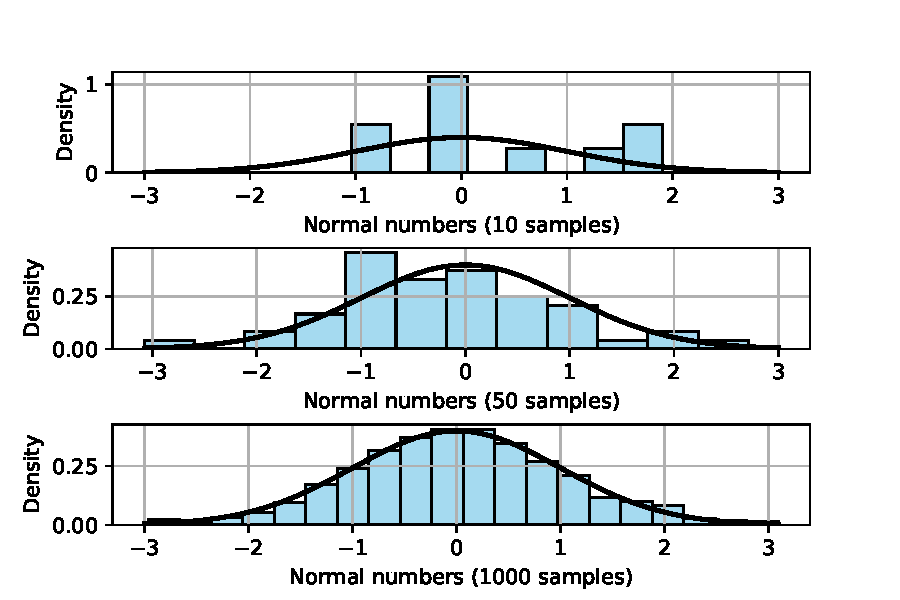
\includegraphics[width = 16 cm]{sources/normalNumbers.pdf}
    \caption{Нормальное распределение \eqref{norm}}
    \label{fig:norm}
\end{figure}
\begin{figure}[H]
    \centering
    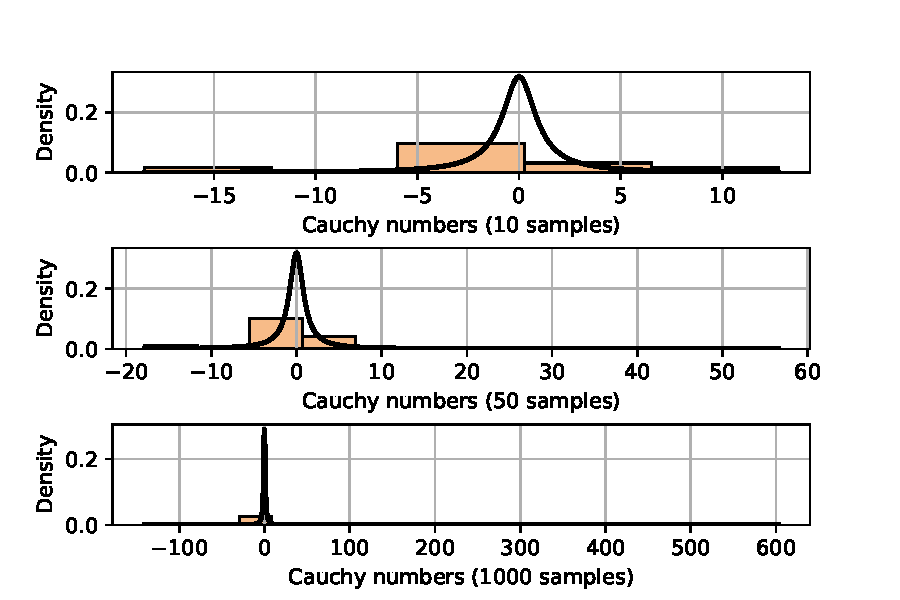
\includegraphics[width = 16 cm]{sources/cauchyNumbers.pdf}
    \caption{Распределение Коши \eqref{cauchy}}
    \label{fig:cauchy}
\end{figure}
\begin{figure}[H]
    \centering
    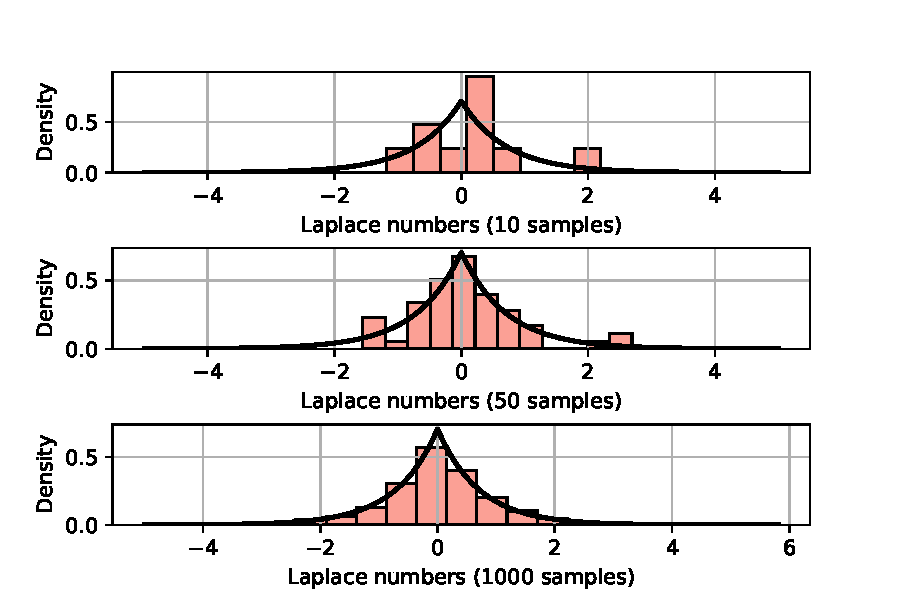
\includegraphics[width = 16 cm]{sources/laplaceNumbers.pdf}
    \caption{Распределение Лапласа \eqref{laplace}}
    \label{fig:laplace}
\end{figure}
\begin{figure}[H]
    \centering
    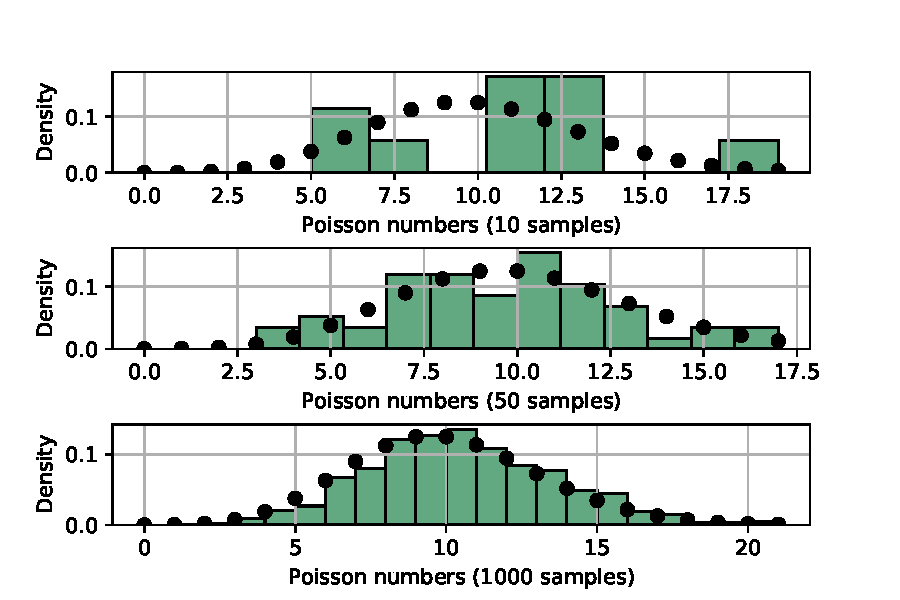
\includegraphics[width = 16 cm]{sources/poissonNumbers.pdf}
    \caption{Распределение Пуассона \eqref{poisson}}
    \label{fig:poisson}
\end{figure}
\begin{figure}[H]
    \centering
    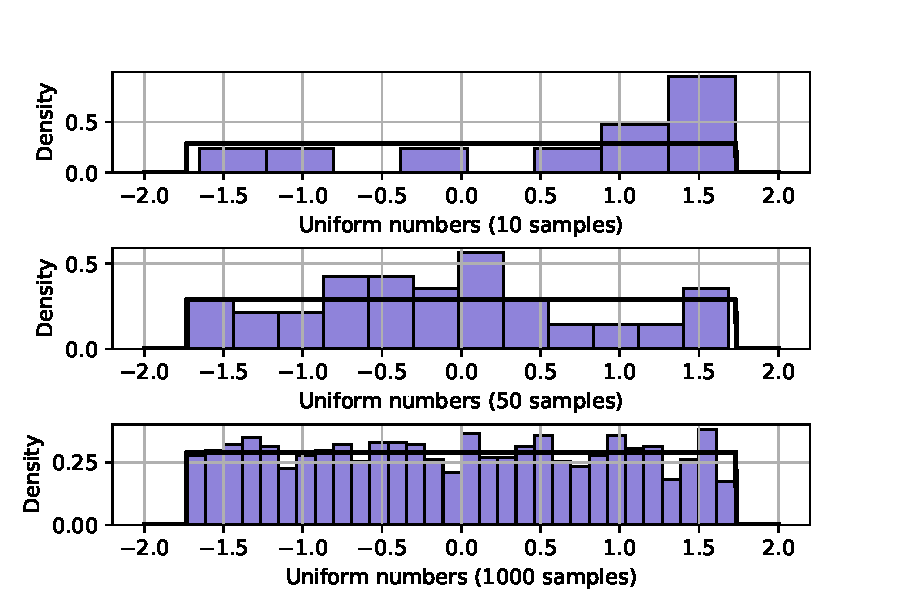
\includegraphics[width = 16 cm]{sources/uniformNumbers.pdf}
    \caption{Равномерное распределение \eqref{uniform}}
    \label{fig:uniform}
\end{figure}
\subsection{Характеристики положения и рассеивания}
\begin{table}[H]
    \centering
    \begin{tabular}{|c|C{2cm}|C{2cm}|C{2cm}|C{2cm}|C{2cm}|}
        \hline
        Normal $n$ = 10& & & & & \\
\hline
 &$\overline{x}\;\eqref{mean}$&$med\;x\;\eqref{med}$&$z_R\;\eqref{exhfsum}$&$z_Q\;\eqref{hfsum}$&$z_{tr}\;\eqref{trmean}$\\
\hline
$E(z)\;\eqref{mean_formula}$&0.00116&0.006212&-0.009496&0.32067&0.28032\\
\hline
$D(z)\;\eqref{variance_formula}$&0.104555&0.143065&0.187496&0.126559&0.122866\\
\hline
$E(z)\pm\sqrt{D(z)}\;\eqref{confint}$&(-0.32219,\newline0.32451)&(-0.372027,\newline0.384451)&(-0.442504,\newline0.423512)&(-0.035081,\newline0.676421)&(-0.070202,\newline0.630842)\\
\hline
 & & & & & \\
\hline
Normal $n$ = 100& & & & & \\
\hline
 &$\overline{x}$&$med\;x$&$z_R$&$z_Q$&$z_{tr}$\\
\hline
$E(z)$&0.001992&-0.000898&-0.009645&0.020634&0.029004\\
\hline
$D(z)$&0.010203&0.014982&0.0945&0.012548&0.012134\\
\hline
$E(z)\pm\sqrt{D(z)}$&(-0.099018,\newline0.103002)&(-0.123299,\newline0.121503)&(-0.317054,\newline0.297764)&(-0.091384,\newline0.132652)&(-0.08115,\newline0.139158)\\
\hline
 & & & & & \\
\hline
Normal $n$ = 1000& & & & & \\
\hline
 &$\overline{x}$&$med\;x$&$z_R$&$z_Q$&$z_{tr}$\\
\hline
$E(z)$&0.001188&0.001011&-0.005252&0.003476&0.003829\\
\hline
$D(z)$&0.001047&0.001673&0.063946&0.001309&0.001279\\
\hline
$E(z)\pm\sqrt{D(z)}$&(-0.031169,\newline0.033545)&(-0.039891,\newline0.041913)&(-0.258127,\newline0.247623)&(-0.032704,\newline0.039656)&(-0.031934,\newline0.039592)\\
\hline

    \end{tabular}
    \caption{Нормальное распределение \eqref{norm}}
    \label{tab:norm}
\end{table}
\begin{table}[H]
    \centering
    \begin{tabular}{|c|C{2cm}|C{2cm}|C{3cm}|C{2cm}|C{2cm}|}
        \hline
        Cauchy $n$ = 10& & & & & \\
\hline
 &$\overline{x}$&$med\;x$&$z_R$&$z_Q$&$z_{tr}$\\
\hline
$E(z)$&-0.186885&-0.009058&-0.998813&1.107276&0.665645\\
\hline
$D(z)$&1220.240065&0.341225&30330.057683&4.39764&1.125819\\
\hline
$E(z)\pm\sqrt{D(z)}$&$-$&(-0.593203,\newline0.575087)&$-$&(-0.989779,\newline3.204331)&(-0.395401,\newline1.726691)\\
\hline
$\widehat{E}(z)$&$-$&0&$-$&0&0\\
\hline
 & & & & & \\
\hline
Cauchy $n$ = 100& & & & & \\
\hline
 &$\overline{x}$&$med\;x$&$z_R$&$z_Q$&$z_{tr}$\\
\hline
$E(z)$&-6.47775&-0.000383&-321.139156&0.026871&0.037994\\
\hline
$D(z)$&18984.933645&0.024235&47380510.140515&0.050965&0.025928\\
\hline
$E(z)\pm\sqrt{D(z)}$&$-$&(-0.156059,\newline0.155293)&$-$&(-0.198883,\newline0.252625)&(-0.123028,\newline0.199016)\\
\hline
$\widehat{E}(z)$&$-$&0&$-$&0&0\\
\hline
 & & & & & \\
\hline
Cauchy $n$ = 1000& & & & & \\
\hline
 &$\overline{x}$&$med\;x$&$z_R$&$z_Q$&$z_{tr}$\\
\hline
$E(z)$&1.893899&-0.000693&960.679479&0.001362&0.003282\\
\hline
$D(z)$&3931.774685&0.00253&981622889.069576&0.005259&0.002648\\
\hline
$E(z)\pm\sqrt{D(z)}$&$-$&(-0.050992,\newline0.049606)&$-$&(-0.071157,\newline0.073881)&(-0.048177,\newline0.054741)\\
\hline
$\widehat{E}(z)$&$-$&0&$-$&0&0\\
\hline

    \end{tabular}
    \caption{Распределение Коши \eqref{cauchy}}
    \label{tab:cauchy}
\end{table}
\begin{table}[H]
    \centering
    \begin{tabular}{|c|C{2cm}|C{2cm}|C{2cm}|C{2cm}|C{2cm}|}
        \hline
        Laplace $n$ = 10& & & & & \\
\hline
 &$\overline{x}$&$med\;x$&$z_R$&$z_Q$&$z_{tr}$\\
\hline
$E(z)$&-0.009415&-0.012622&-0.024343&0.300827&0.227097\\
\hline
$D(z)$&0.102728&0.072915&0.430623&0.118063&0.081524\\
\hline
$E(z)\pm\sqrt{D(z)}$&(-0.329927,\newline0.311097)&(-0.28265,\newline0.257406)&(-0.680562,\newline0.631876)&(-0.042776,\newline0.64443)&(-0.058427,\newline0.512621)\\
\hline
 & & & & & \\
\hline
Laplace $n$ = 100& & & & & \\
\hline
 &$\overline{x}$&$med\;x$&$z_R$&$z_Q$&$z_{tr}$\\
\hline
$E(z)$&0.00684&0.005635&0.029287&0.019885&0.024766\\
\hline
$D(z)$&0.010063&0.006018&0.401845&0.010201&0.006588\\
\hline
$E(z)\pm\sqrt{D(z)}$&(-0.093475,\newline0.107155)&(-0.071941,\newline0.083211)&(-0.604625,\newline0.663199)&(-0.081115,\newline0.120885)&(-0.0564,\newline0.105932)\\
\hline
 & & & & & \\
\hline
Laplace $n$ = 1000& & & & & \\
\hline
 &$\overline{x}$&$med\;x$&$z_R$&$z_Q$&$z_{tr}$\\
\hline
$E(z)$&-0.00239&-0.000474&-0.034909&-0.000289&0.000806\\
\hline
$D(z)$&0.001037&0.000503&0.387083&0.001029&0.000606\\
\hline
$E(z)\pm\sqrt{D(z)}$&(-0.034592,\newline0.029812)&(-0.022902,\newline0.021954)&(-0.657069,\newline0.587251)&(-0.032367,\newline0.031789)&(-0.023811,\newline0.025423)\\
\hline

    \end{tabular}
    \caption{Распределение Лапласа \eqref{laplace}}
    \label{tab:laplace}
\end{table}
\begin{table}[H]
    \centering
    \begin{tabular}{|c|C{2cm}|C{2cm}|C{2cm}|C{2cm}|C{2cm}|}
        \hline
        Poisson $n$ = 10& & & & & \\
\hline
 &$\overline{x}$&$med\;x$&$z_R$&$z_Q$&$z_{tr}$\\
\hline
$E(z)$&9.994&9.8345&10.32&10.9715&10.7695\\
\hline
$D(z)$&1.052584&1.46836&1.9546&1.385938&1.281564\\
\hline
$E(z)\pm\sqrt{D(z)}$&(8.968045,\newline11.019955)&(8.622741,\newline11.046259)&(8.92193,\newline11.71807)&(9.794241,\newline12.148759)&(9.637438,\newline11.901562)\\
\hline
 & & & & & \\
\hline
Poisson $n$ = 100& & & & & \\
\hline
 &$\overline{x}$&$med\;x$&$z_R$&$z_Q$&$z_{tr}$\\
\hline
$E(z)$&10.00871&9.8785&10.933&9.9665&9.95862\\
\hline
$D(z)$&0.100729&0.202488&1.077011&0.151628&0.118006\\
\hline
$E(z)\pm\sqrt{D(z)}$&(9.691332,\newline10.326088)&(9.428513,\newline10.328487)&(9.895209,\newline11.970791)&(9.577106,\newline10.355894)&(9.6151,\newline10.30214)\\
\hline
 & & & & & \\
\hline
Poisson $n$ = 1000& & & & & \\
\hline
 &$\overline{x}$&$med\;x$&$z_R$&$z_Q$&$z_{tr}$\\
\hline
$E(z)$&10.005459&9.999&11.714&9.9975&9.870534\\
\hline
$D(z)$&0.010818&0.000999&0.699704&0.002244&0.011732\\
\hline
$E(z)\pm\sqrt{D(z)}$&(9.901449,\newline10.109469)&(9.967393,\newline10.030607)&(10.877517,\newline12.550483)&(9.950129,\newline10.044871)&(9.76222,\newline9.978848)\\
\hline

    \end{tabular}
    \caption{Распределение Пуассона \eqref{poisson}}
    \label{tab:poisson}
\end{table}
\begin{table}[H]
    \centering
    \begin{tabular}{|c|C{2cm}|C{2cm}|C{2cm}|C{2cm}|C{2cm}|}
        \hline
        Uniform $n$ = 10& & & & & \\
\hline
 &$\overline{x}$&$med\;x$&$z_R$&$z_Q$&$z_{tr}$\\
\hline
$E(z)$&0.00987&0.007138&0.013105&0.324796&0.324069\\
\hline
$D(z)$&0.103187&0.230005&0.046384&0.131897&0.154831\\
\hline
$E(z)\pm\sqrt{D(z)}$&(-0.311357,\newline0.331097)&(-0.47245,\newline0.486726)&(-0.202264,\newline0.228474)&(-0.03838,\newline0.687972)&(-0.069417,\newline0.717555)\\
\hline
 & & & & & \\
\hline
Uniform $n$ = 100& & & & & \\
\hline
 &$\overline{x}$&$med\;x$&$z_R$&$z_Q$&$z_{tr}$\\
\hline
$E(z)$&-0.002077&-0.001152&0.000943&0.014305&0.030867\\
\hline
$D(z)$&0.009315&0.027453&0.000563&0.013355&0.017855\\
\hline
$E(z)\pm\sqrt{D(z)}$&(-0.098591,\newline0.094437)&(-0.166841,\newline0.164537)&(-0.022785,\newline0.024671)&(-0.101259,\newline0.129869)&(-0.102756,\newline0.16449)\\
\hline
 & & & & & \\
\hline
Uniform $n$ = 1000& & & & & \\
\hline
 &$\overline{x}$&$med\;x$&$z_R$&$z_Q$&$z_{tr}$\\
\hline
$E(z)$&0.000581&0.001917&2e-05&0.002004&0.005029\\
\hline
$D(z)$&0.000994&0.002952&6e-06&0.001484&0.001998\\
\hline
$E(z)\pm\sqrt{D(z)}$&(-0.030947,\newline0.032109)&(-0.052415,\newline0.056249)&(-0.002429,\newline0.002469)&(-0.036519,\newline0.040527)&(-0.03967,\newline0.049728)\\
\hline

    \end{tabular}
    \caption{Равномерное распределение \eqref{uniform}}
    \label{tab:uniform}
\end{table}
\subsection{Ящики с <<усами>>}
\begin{figure}[H]
    \centering
    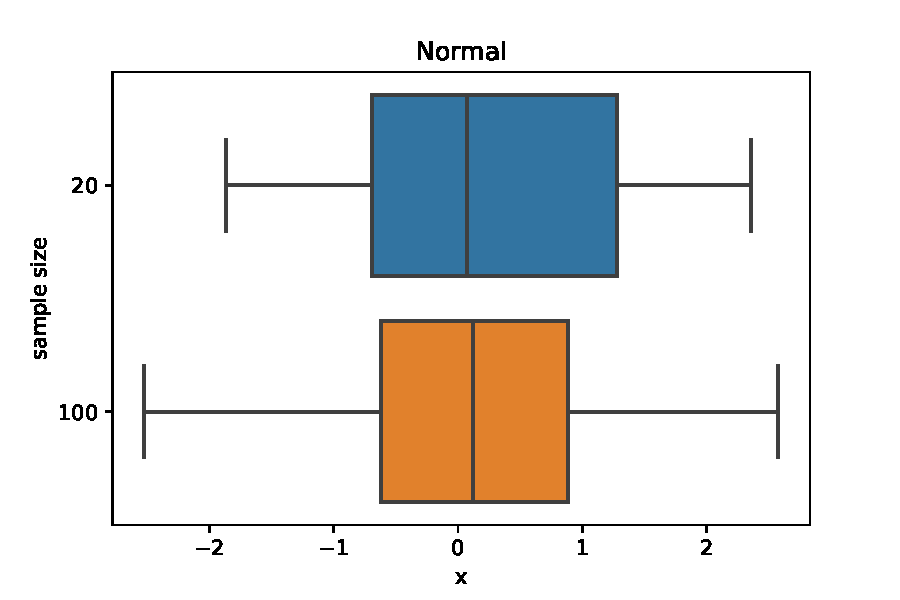
\includegraphics[width = 16 cm]{sources/NormalBox.pdf}
    \caption{Нормальное распределение \eqref{norm}}
    \label{fig:normBox}
\end{figure}
\begin{figure}[H]
    \centering
    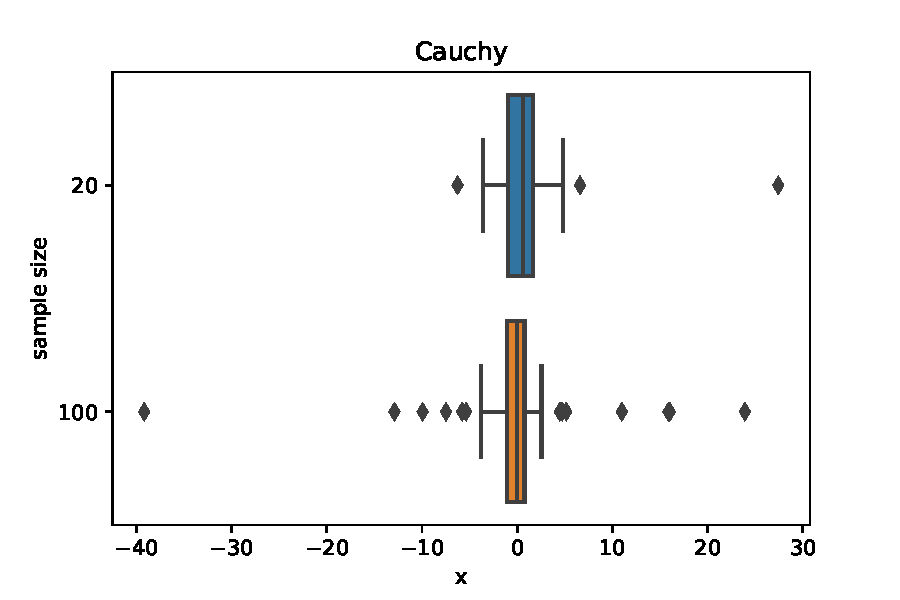
\includegraphics[width = 16 cm]{sources/CauchyBox.pdf}
    \caption{Распределение Коши \eqref{cauchy}}
    \label{fig:cauchyBox}
\end{figure}
\begin{figure}[H]
    \centering
    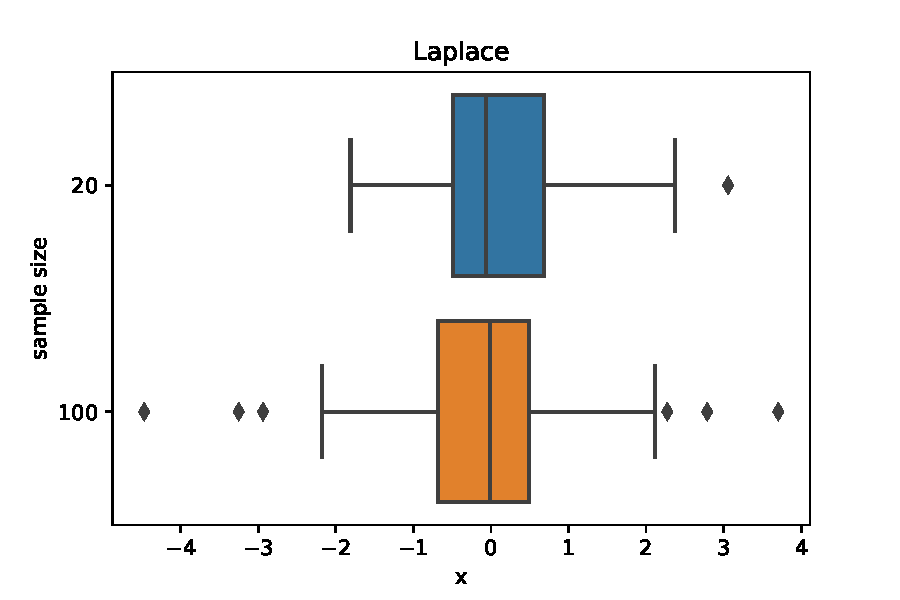
\includegraphics[width = 16 cm]{sources/LaplaceBox.pdf}
    \caption{Распределение Лапласа \eqref{laplace}}
    \label{fig:laplaceBox}
\end{figure}
\begin{figure}[H]
    \centering
    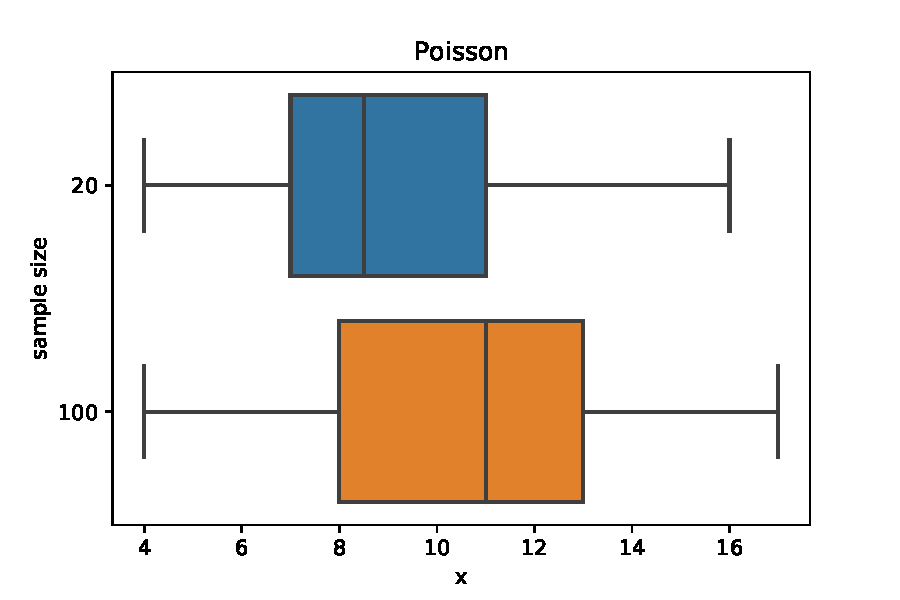
\includegraphics[width = 16 cm]{sources/PoissonBox.pdf}
    \caption{Распределение Пуассона \eqref{poisson}}
    \label{fig:poissonBox}
\end{figure}
\begin{figure}[H]
    \centering
    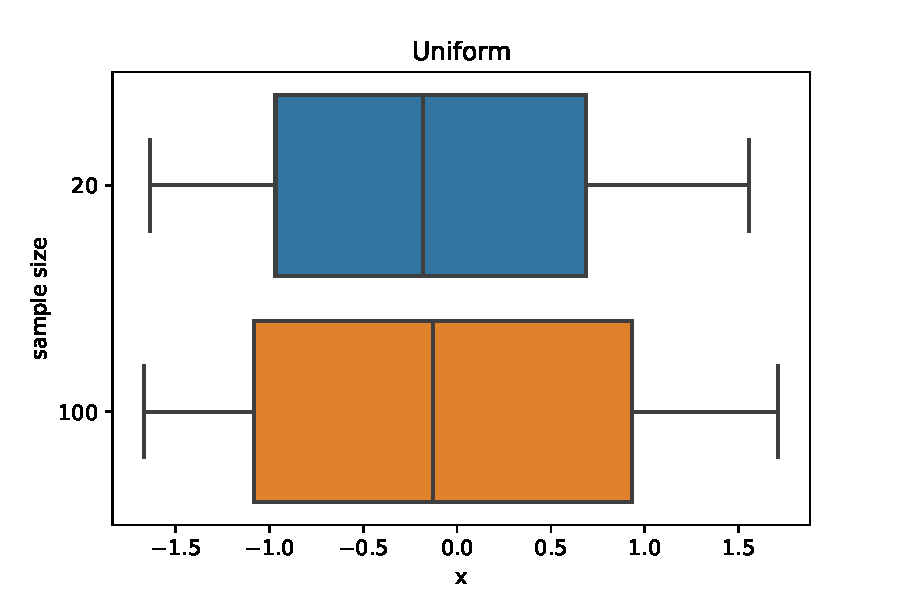
\includegraphics[width = 16 cm]{sources/UniformBox.pdf}
    \caption{Равномерное распределение \eqref{uniform}}
    \label{fig:uniformBox}
\end{figure}
\subsection{Доля выбросов}
\begin{table}[H]
    \centering
    \begin{tabular}{|c|c|}
        \hline
        Выборка&Доля выбросов\\\hline Normal $n$ = 20&0.017\\\hline Normal $n$ = 100&0.009\\\hline Cauchy $n$ = 20&0.146\\\hline Cauchy $n$ = 100&0.154\\\hline Laplace $n$ = 20&0.065\\\hline Laplace $n$ = 100&0.063\\\hline Poisson $n$ = 20&0.018\\\hline Poisson $n$ = 100&0.009\\\hline Uniform $n$ = 20&0.002\\\hline Uniform $n$ = 100&0.0\\\hline 
    \end{tabular}
    \caption{Доля выбросов}
    \label{tab:outlierstests}
\end{table}
\subsection{Теоретическая вероятность выбросов}
\begin{table}[H]
    \centering
    \begin{tabular}{|c|c|c|c|c|c|}
        \hline
        Распределение&$Q^{\text{т}}_1$&$Q^{\text{т}}_3$&$X^{\text{т}}_1\;\eqref{whiskers}$&$X^{\text{т}}_2\;\eqref{whiskers}$&$P^{\text{т}}_{\text{в}}\;\eqref{abscontprob},\;\eqref{discrprob}$\\
\hline
Нормальное распределение&-0.674&0.674&-2.698&2.698&0.007\\
\hline
Распределение Коши&-1.0&1.0&-4.0&4.0&0.156\\
\hline
Распределение Лапласа&-0.49&0.49&-1.961&1.961&0.062\\
\hline
Распределение Пуассона&8.0&12.0&2.0&18.0&0.008\\
\hline
Равномерное распределение&-0.866&0.866&-3.464&3.464&0.0\\
\hline

    \end{tabular}
    \caption{Теоретическая вероятность выбросов}
    \label{tab:outlierstheory}
\end{table}
\subsection{Эмпирическая функция распределения}
\begin{figure}[H]
    \centering
    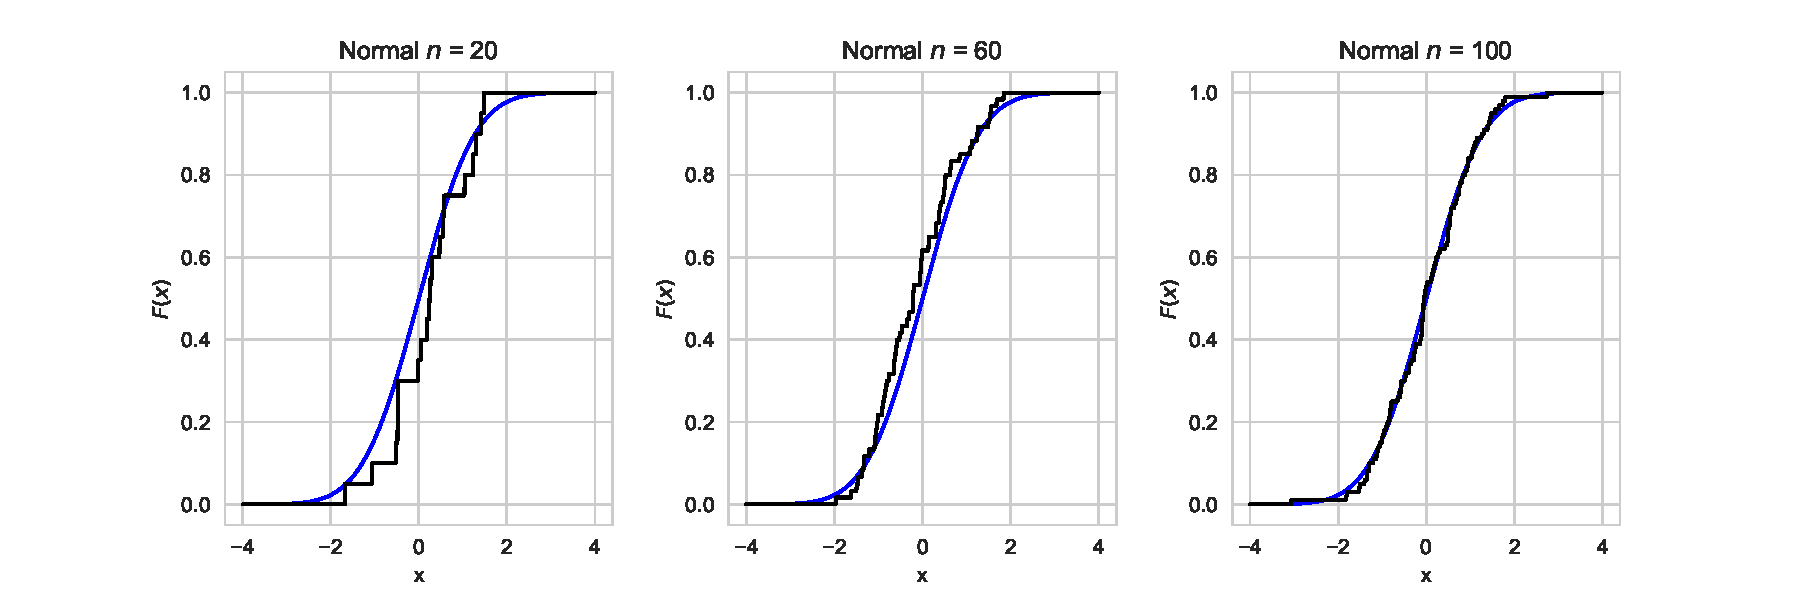
\includegraphics[width = 16 cm]{sources/normalECDF.pdf}
    \caption{Нормальное распределение \eqref{norm}}
    \label{fig:normECDF}
\end{figure}
\begin{figure}[H]
    \centering
    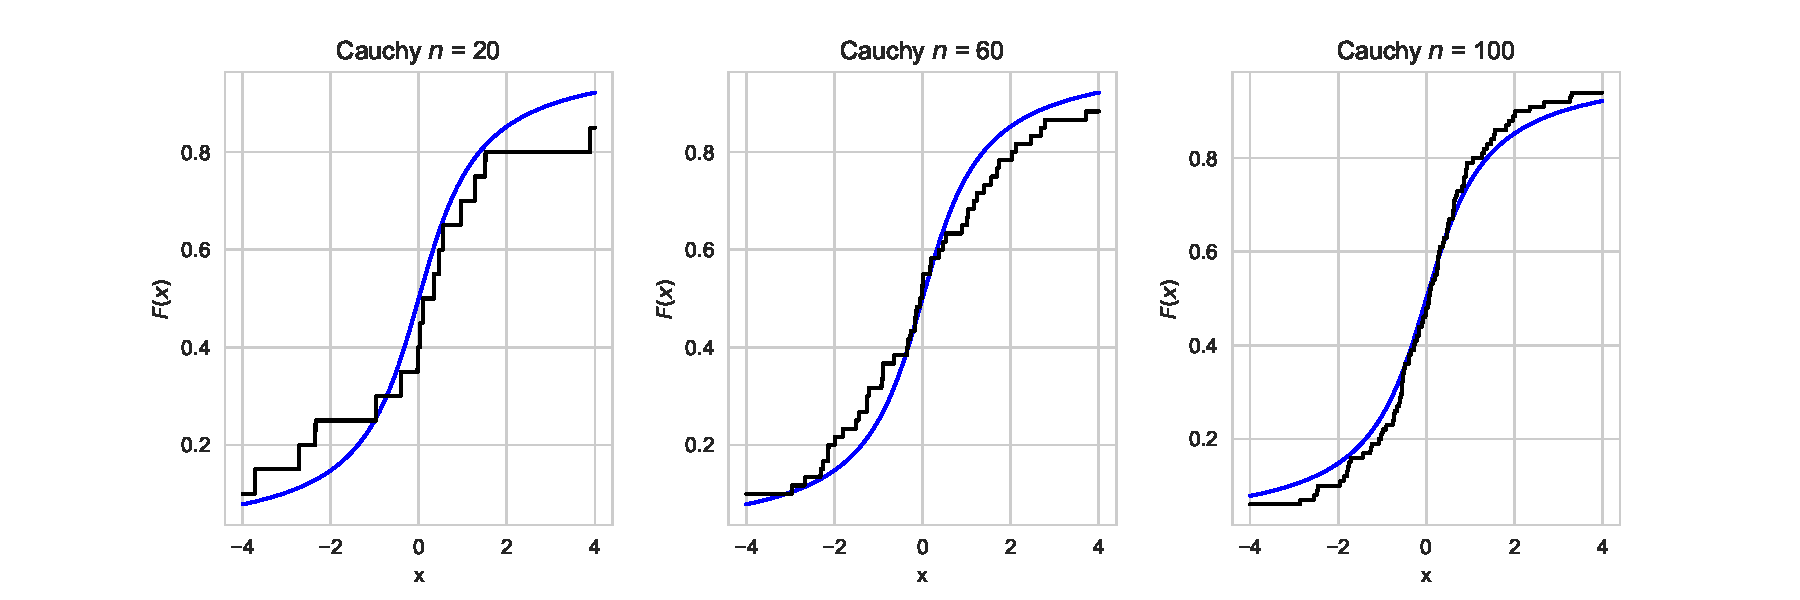
\includegraphics[width = 16 cm]{sources/cauchyECDF.pdf}
    \caption{Распределение Коши \eqref{cauchy}}
    \label{fig:cauchyECDF}
\end{figure}
\begin{figure}[H]
    \centering
    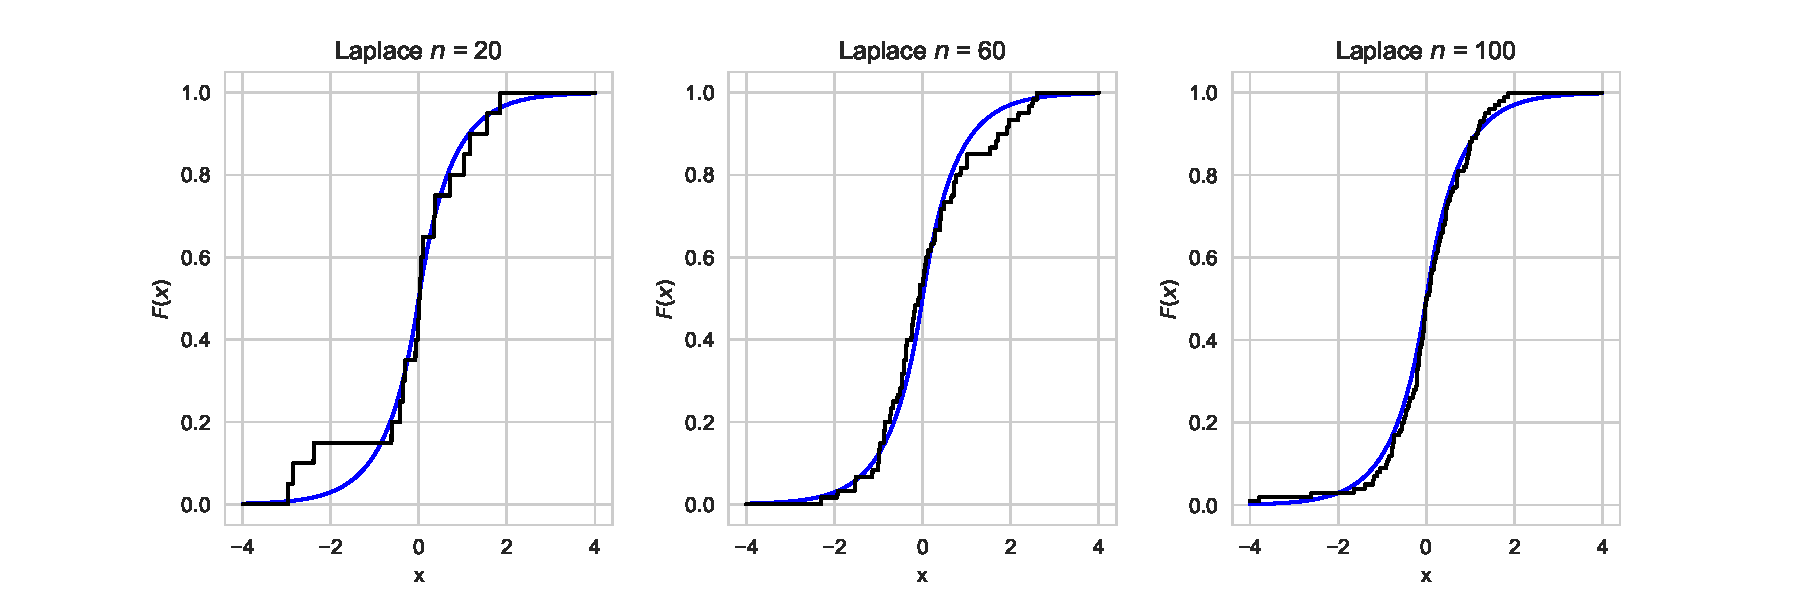
\includegraphics[width = 16 cm]{sources/laplaceECDF.pdf}
    \caption{Распределение Лапласа \eqref{laplace}}
    \label{fig:laplaceECDF}
\end{figure}
\begin{figure}[H]
    \centering
    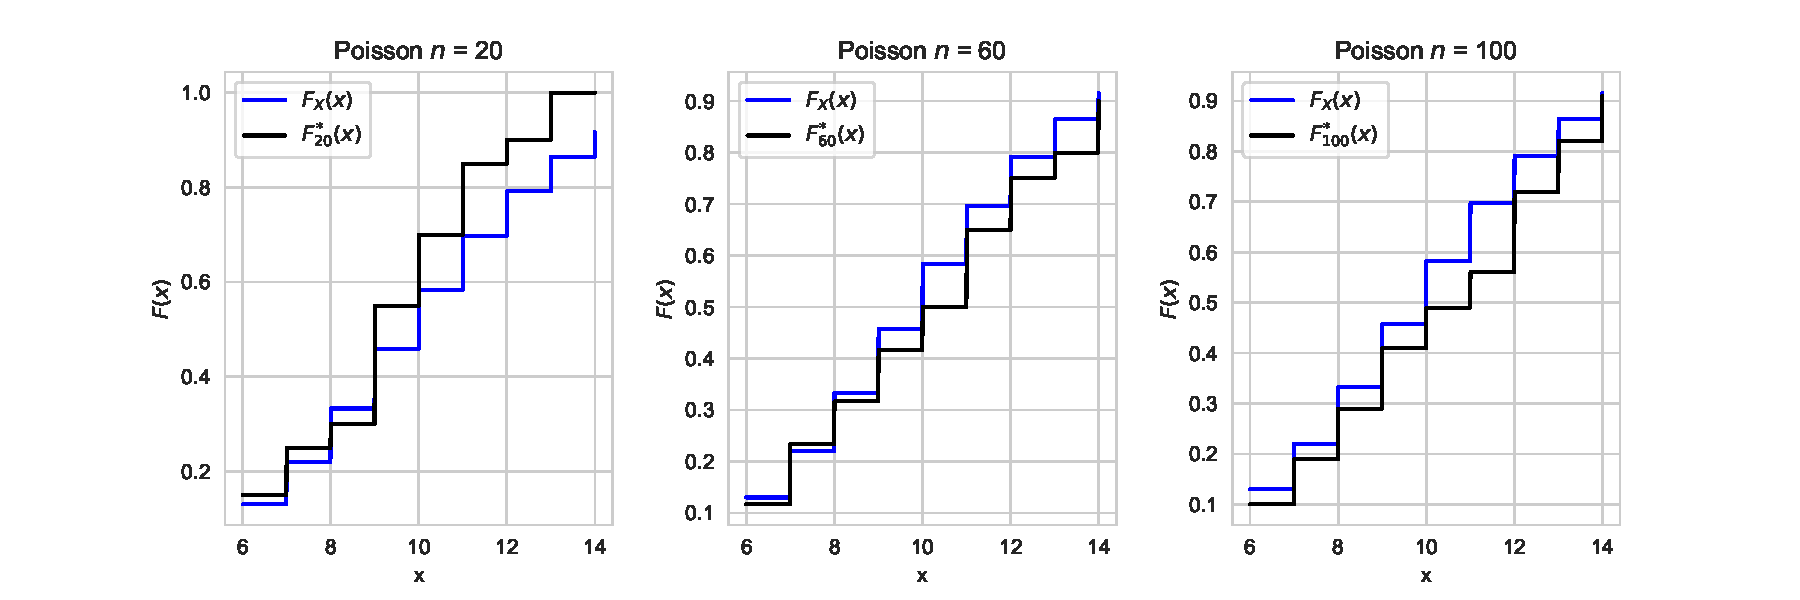
\includegraphics[width = 16 cm]{sources/poissonECDF.pdf}
    \caption{Распределение Пуассона \eqref{poisson}}
    \label{fig:poissonECDF}
\end{figure}
\begin{figure}[H]
    \centering
    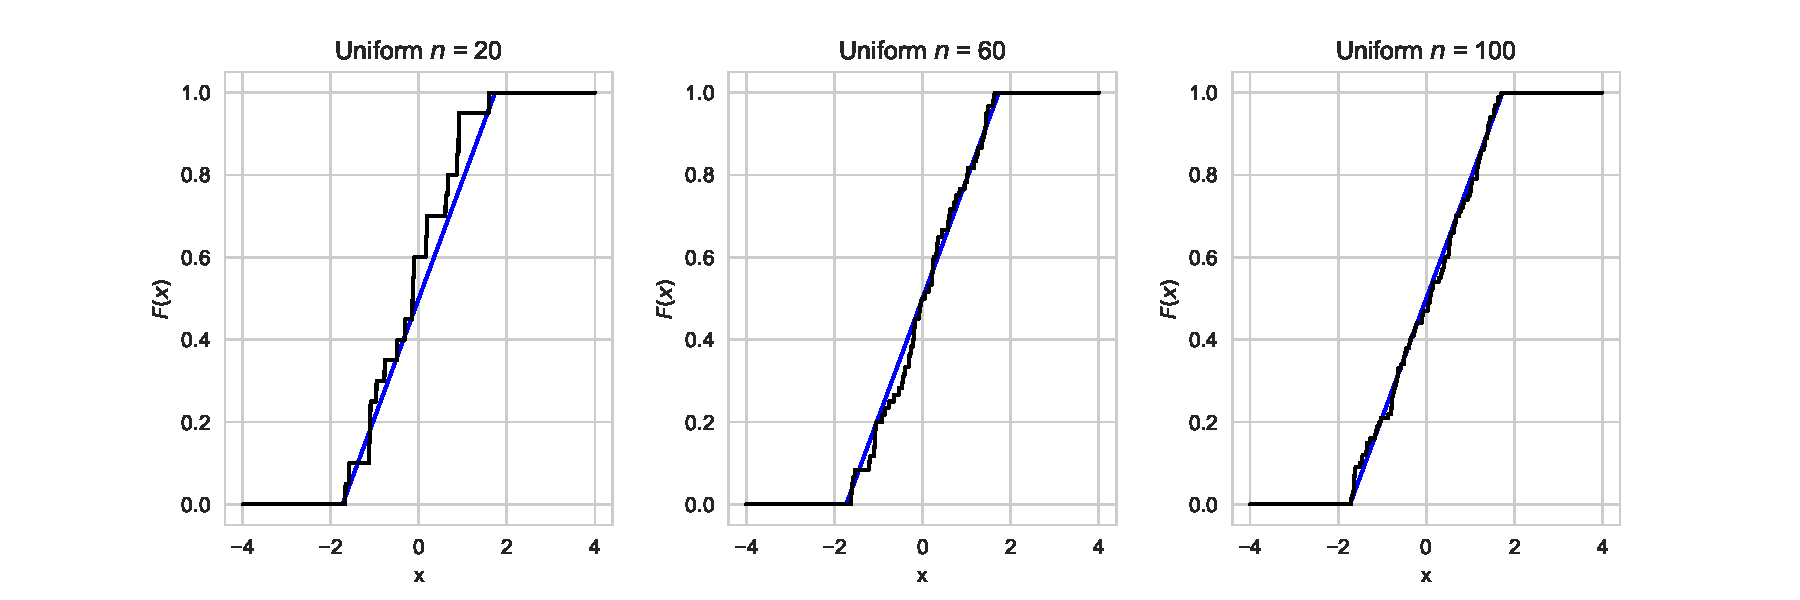
\includegraphics[width = 16 cm]{sources/uniformECDF.pdf}
    \caption{Равномерное распределение \eqref{uniform}}
    \label{fig:uniformECDF}
\end{figure}
\subsection{Ядерные оценки плотности распределения}
\subsubsection{Нормальное распределение}
\begin{figure}[H]
    \centering
    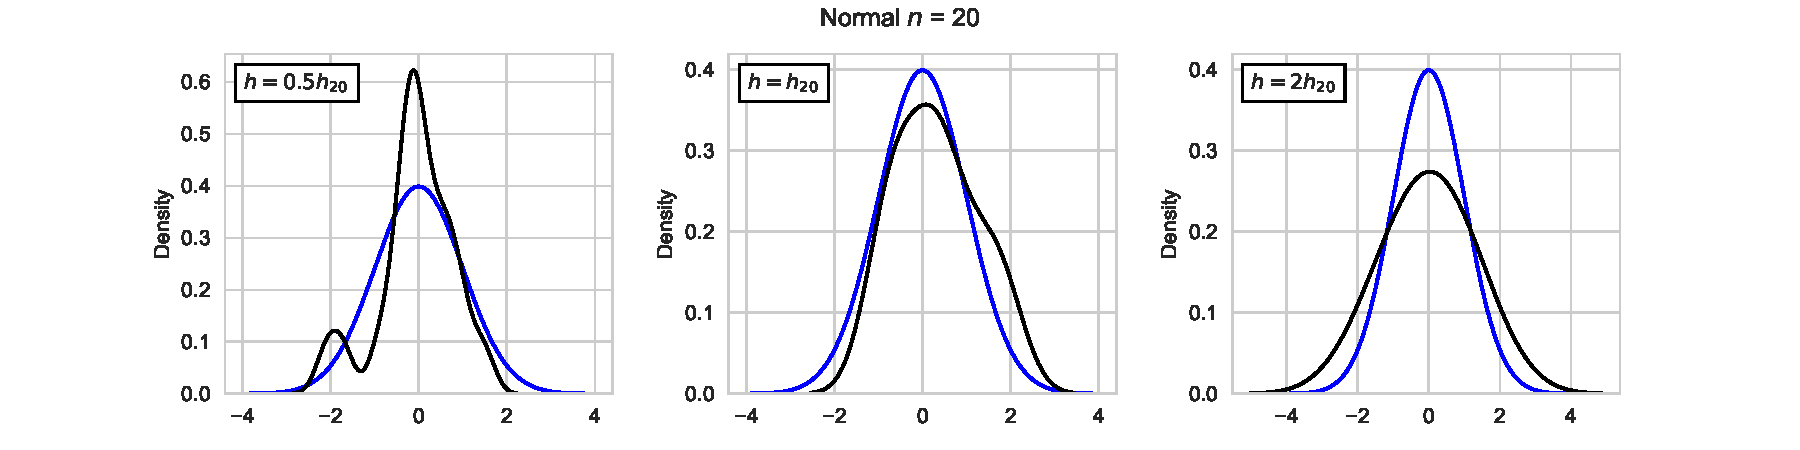
\includegraphics[width = 16 cm]{sources/normalKde20.pdf}
    \caption{Нормальное распределение \eqref{norm}, $n = 20$}
    \label{fig:normKDE20}
\end{figure}
\begin{figure}[H]
    \centering
    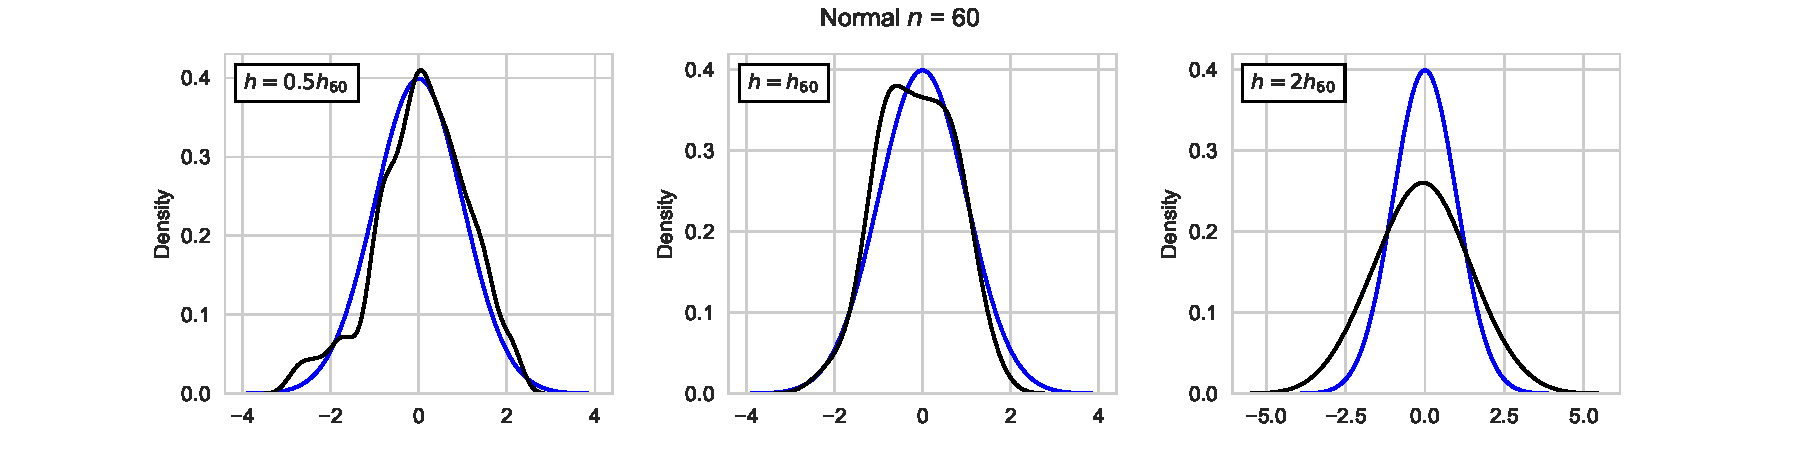
\includegraphics[width = 16 cm]{sources/normalKde60.pdf}
    \caption{Нормальное распределение \eqref{norm}, $n = 60$}
    \label{fig:normKDE60}
\end{figure}
\begin{figure}[H]
    \centering
    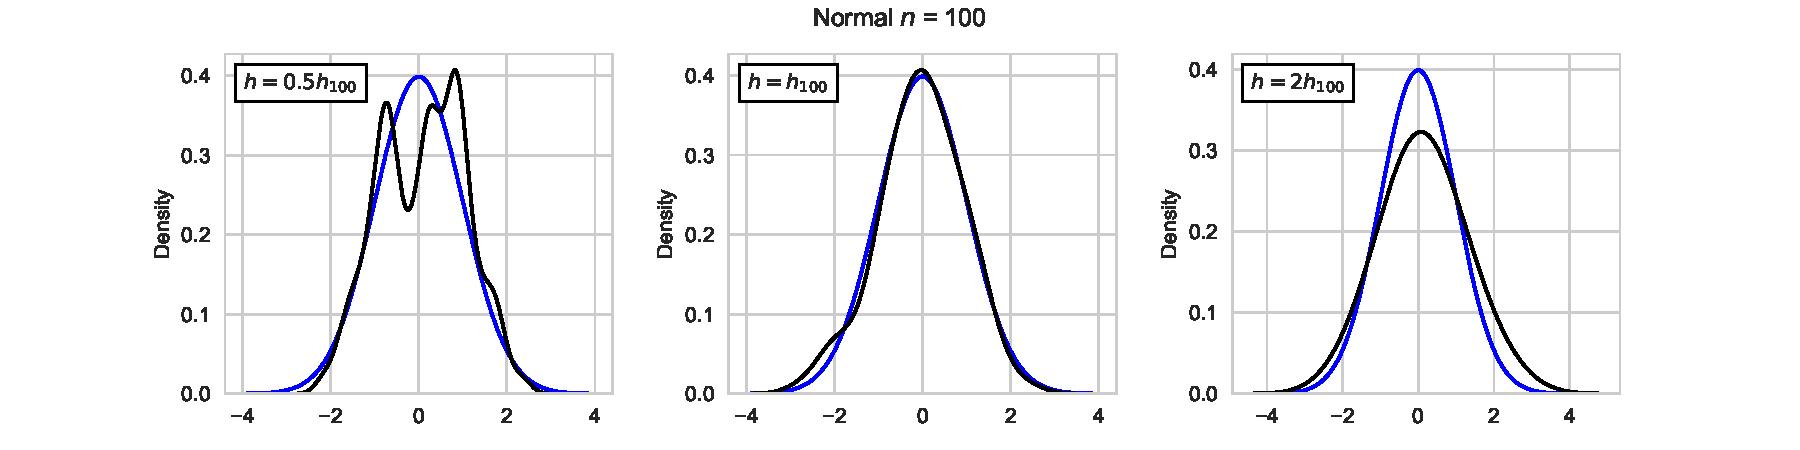
\includegraphics[width = 16 cm]{sources/normalKde100.pdf}
    \caption{Нормальное распределение \eqref{norm}, $n = 100$}
    \label{fig:normKDE100}
\end{figure}
\subsubsection{Распределение Коши}
\begin{figure}[H]
    \centering
    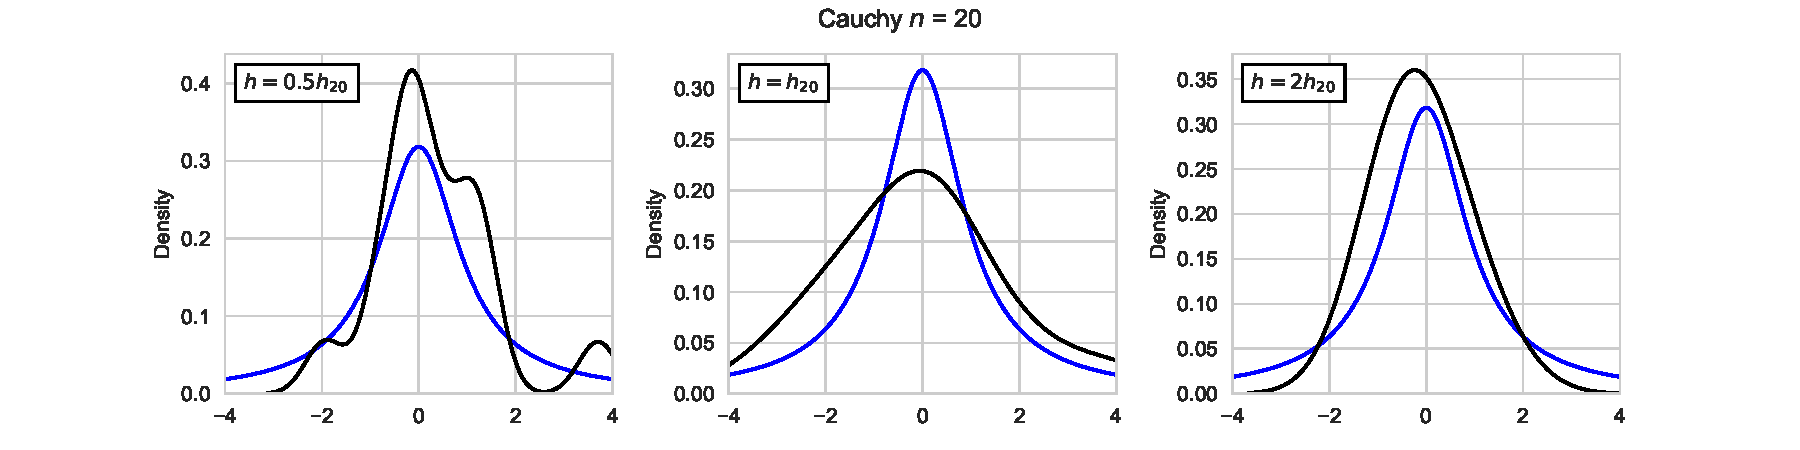
\includegraphics[width = 16 cm]{sources/cauchyKde20.pdf}
    \caption{Распределение Коши \eqref{cauchy}, $n = 20$}
    \label{fig:cauchyKDE20}
\end{figure}
\begin{figure}[H]
    \centering
    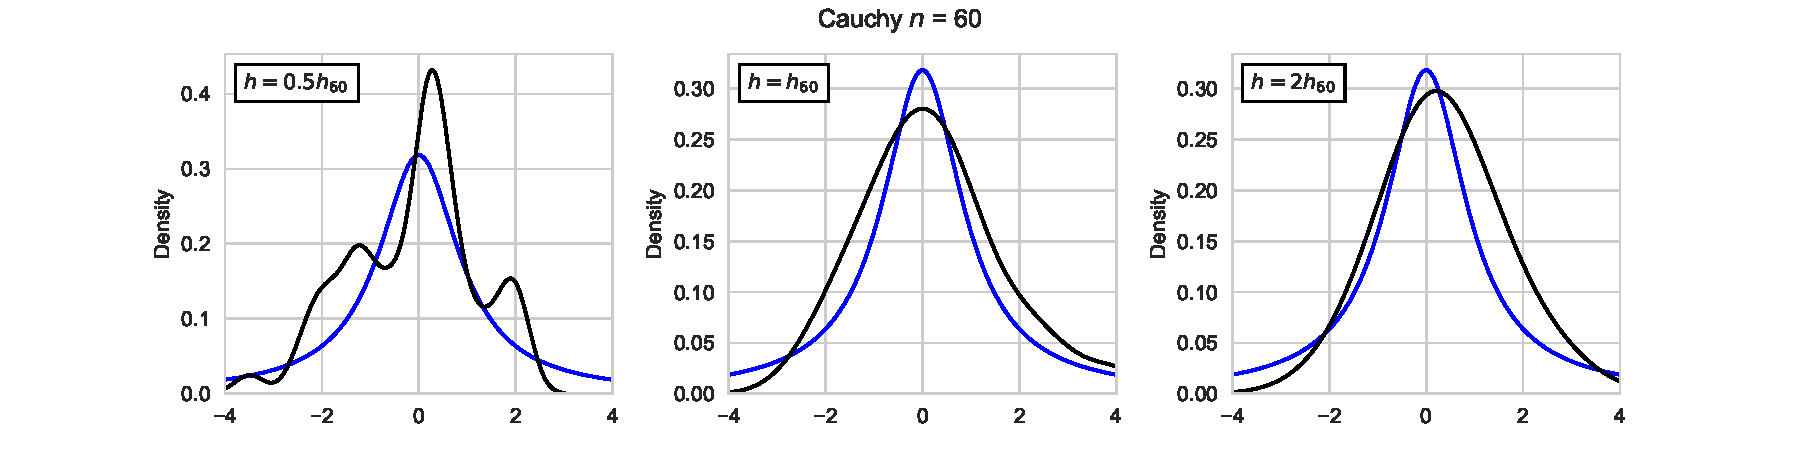
\includegraphics[width = 16 cm]{sources/cauchyKde60.pdf}
    \caption{Распределение Коши \eqref{cauchy}, $n = 60$}
    \label{fig:cauchyKDE60}
\end{figure}
\begin{figure}[H]
    \centering
    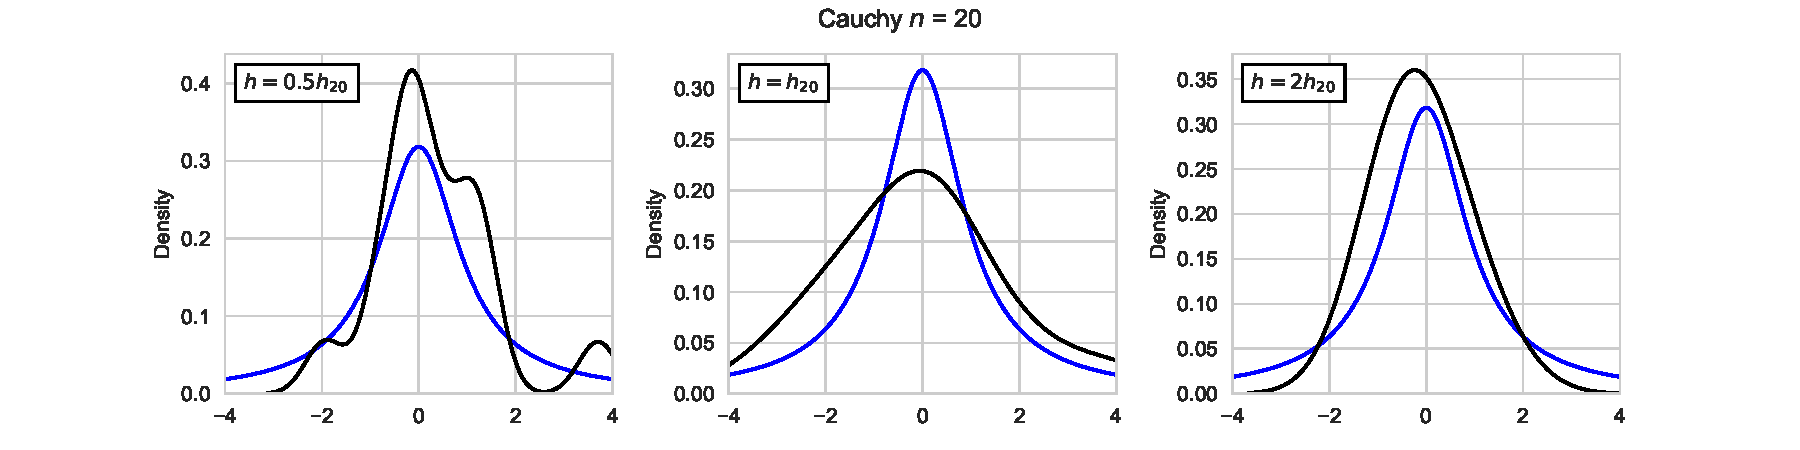
\includegraphics[width = 16 cm]{sources/cauchyKde20.pdf}
    \caption{Распределение Коши \eqref{cauchy}, $n = 100$}
    \label{fig:cauchyKDE100}
\end{figure}
\subsubsection{Распределение Лапласа}
\begin{figure}[H]
    \centering
    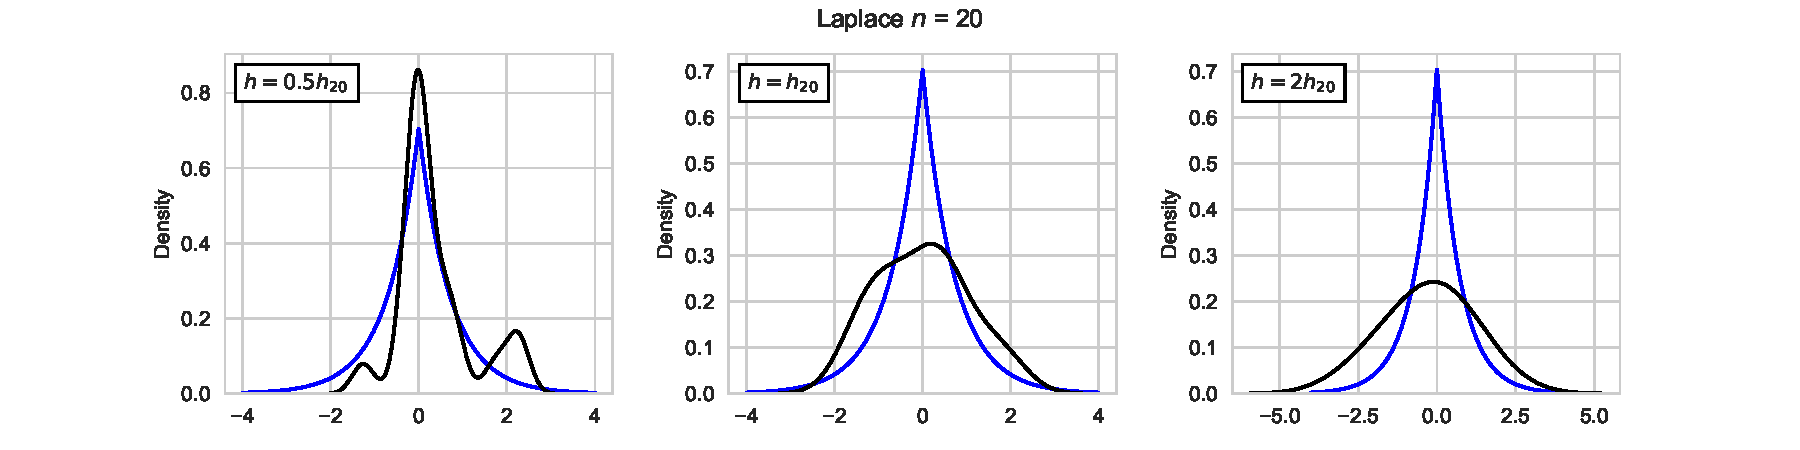
\includegraphics[width = 16 cm]{sources/laplaceKde20.pdf}
    \caption{Распределение Лапласа \eqref{laplace}, $n = 20$}
    \label{fig:laplaceKDE20}
\end{figure}
\begin{figure}[H]
    \centering
    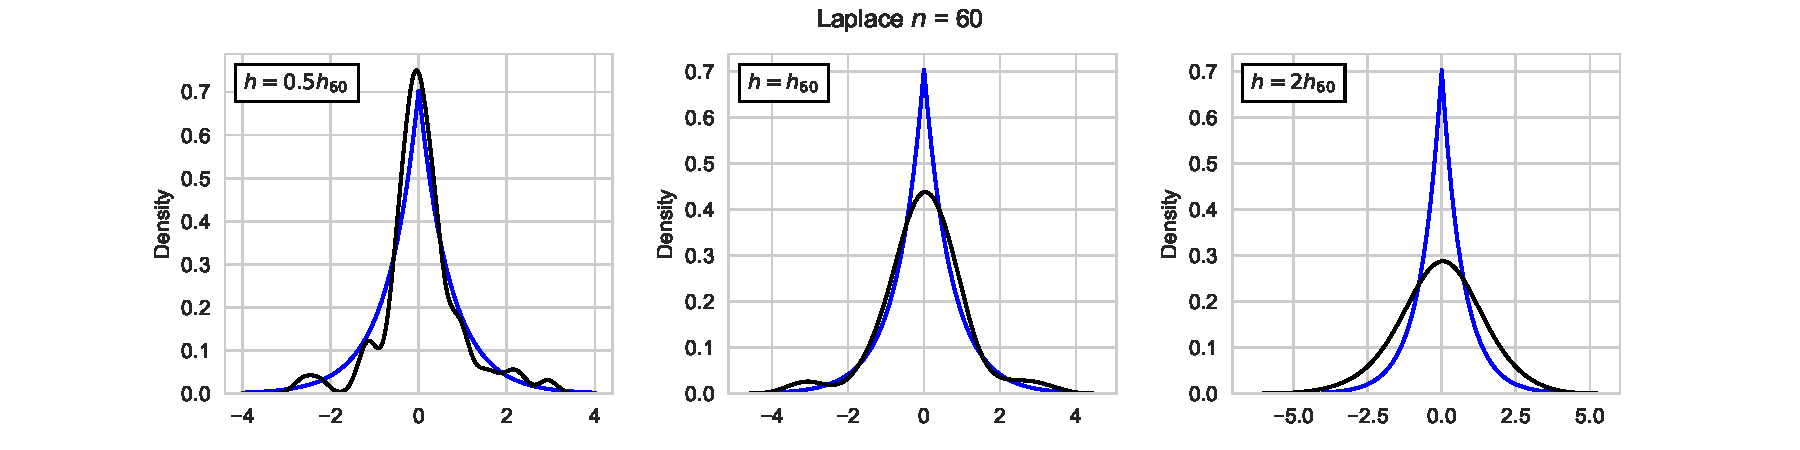
\includegraphics[width = 16 cm]{sources/laplaceKde60.pdf}
    \caption{Распределение Лапласа \eqref{laplace}, $n = 60$}
    \label{fig:laplaceKDE60}
\end{figure}
\begin{figure}[H]
    \centering
    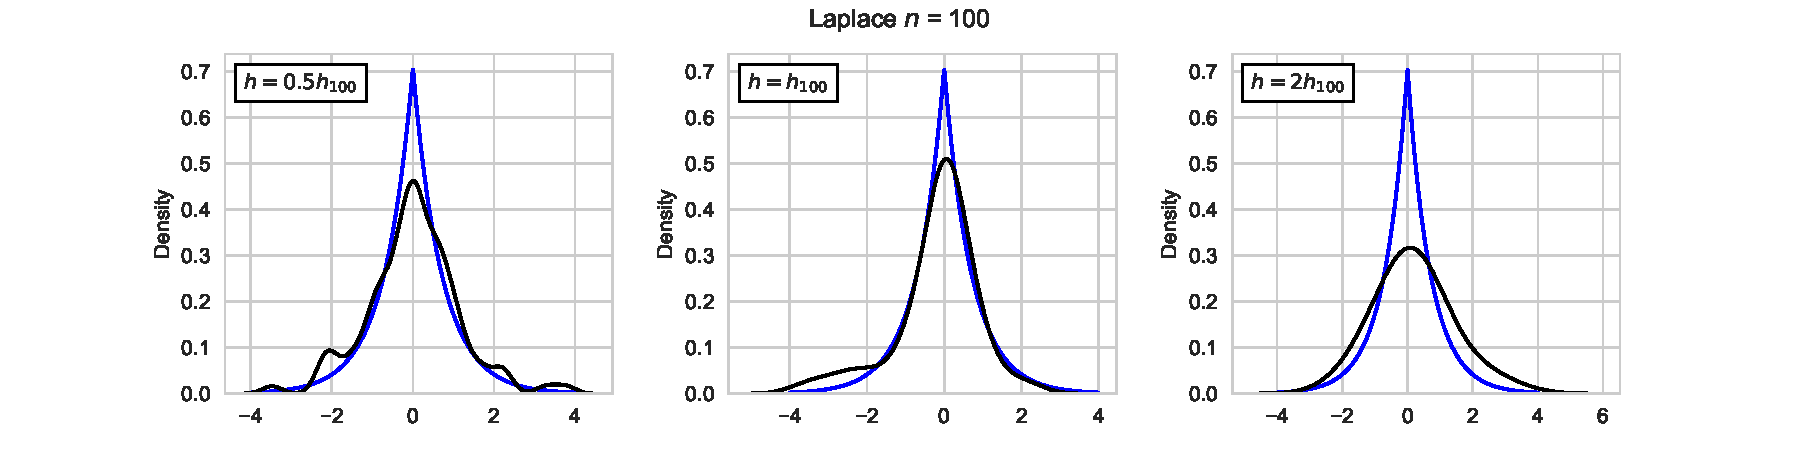
\includegraphics[width = 16 cm]{sources/laplaceKde100.pdf}
    \caption{Распределение Лапласа \eqref{laplace}, $n = 100$}
    \label{fig:laplaceKDE100}
\end{figure}
\subsubsection{Распределение Пуассона}
\begin{figure}[H]
    \centering
    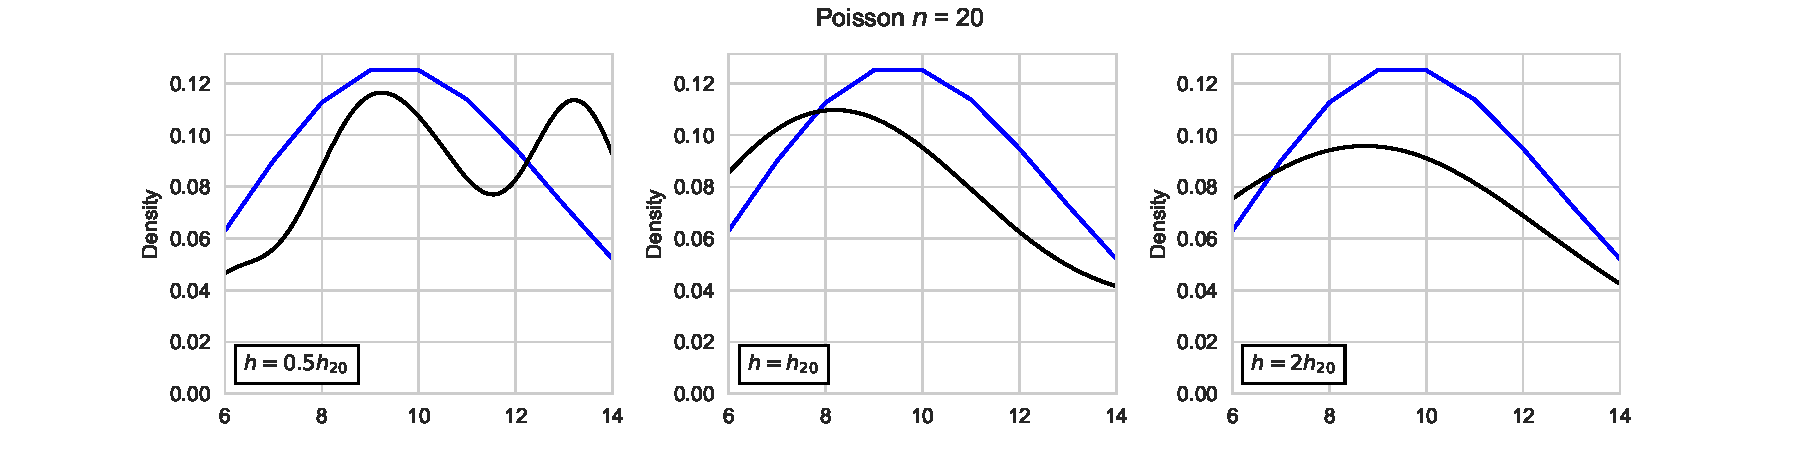
\includegraphics[width = 16 cm]{sources/poisKde20.pdf}
    \caption{Распределение Пуассона \eqref{poisson}, $n = 20$}
    \label{fig:poissonKDE20}
\end{figure}
\begin{figure}[H]
    \centering
    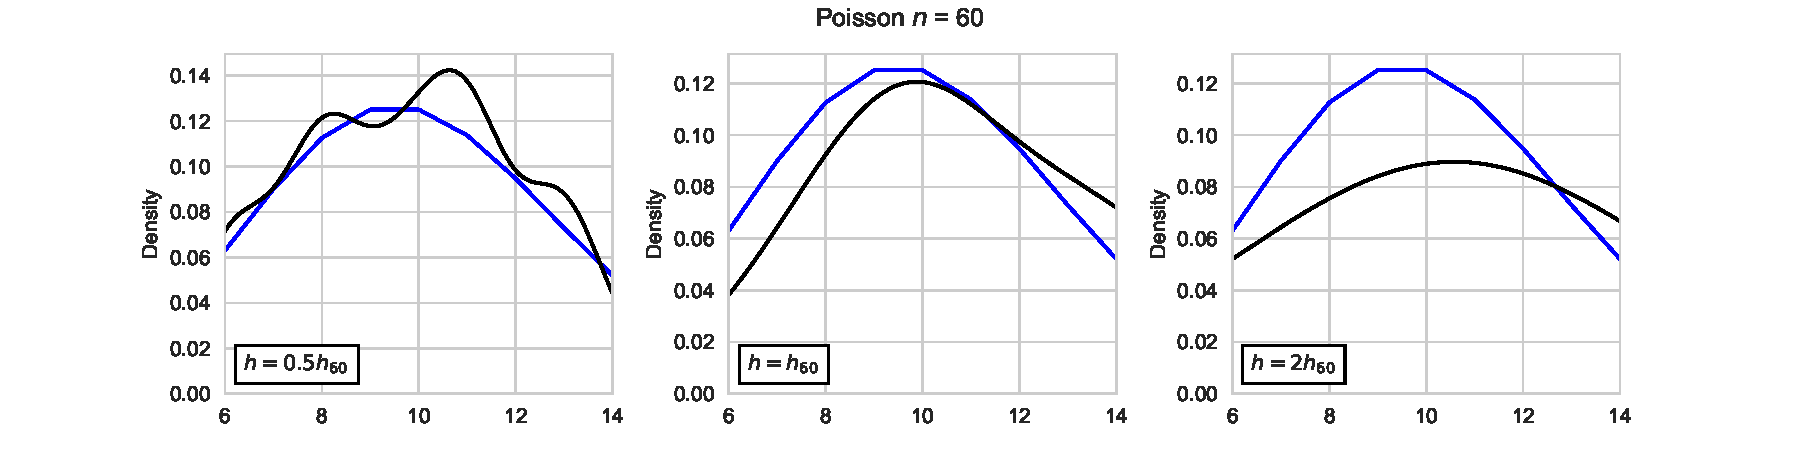
\includegraphics[width = 16 cm]{sources/poisKde60.pdf}
    \caption{Распределение Пуассона \eqref{poisson}, $n = 60$}
    \label{fig:poissonKDE60}
\end{figure}
\begin{figure}[H]
    \centering
    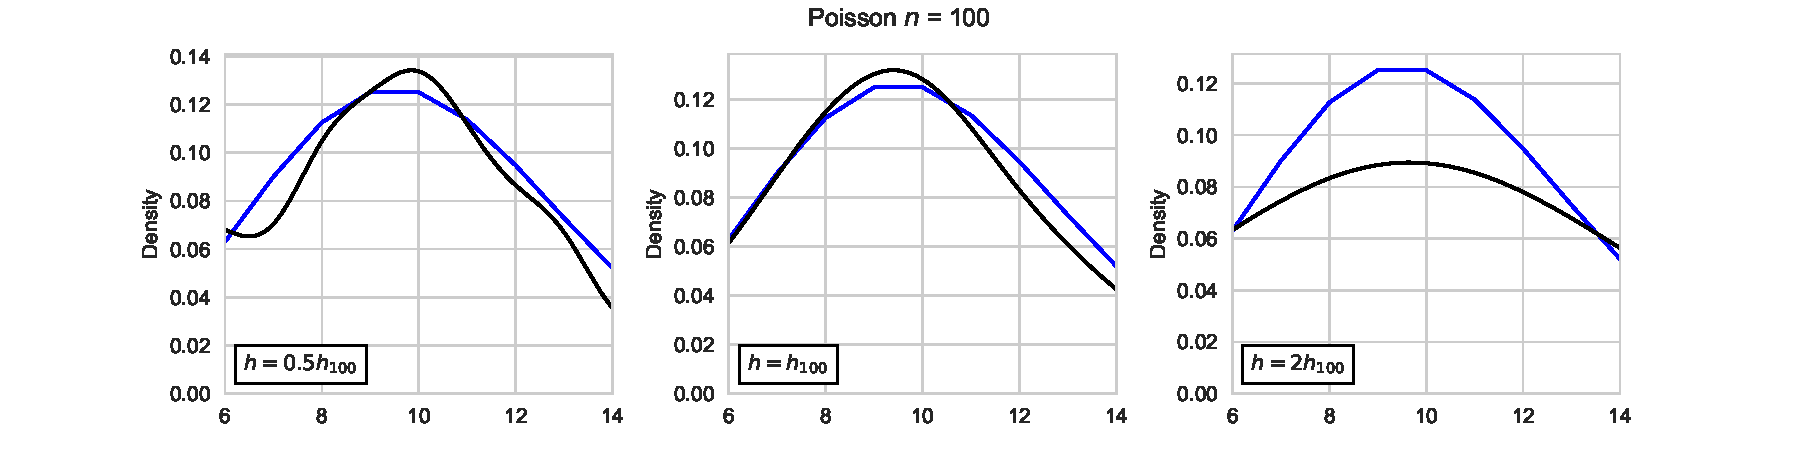
\includegraphics[width = 16 cm]{sources/poisKde100.pdf}
    \caption{Распределение Пуассона \eqref{poisson}, $n = 100$}
    \label{fig:poissonKDE100}
\end{figure}
\subsubsection{Равномерное распределение}
\begin{figure}[H]
    \centering
    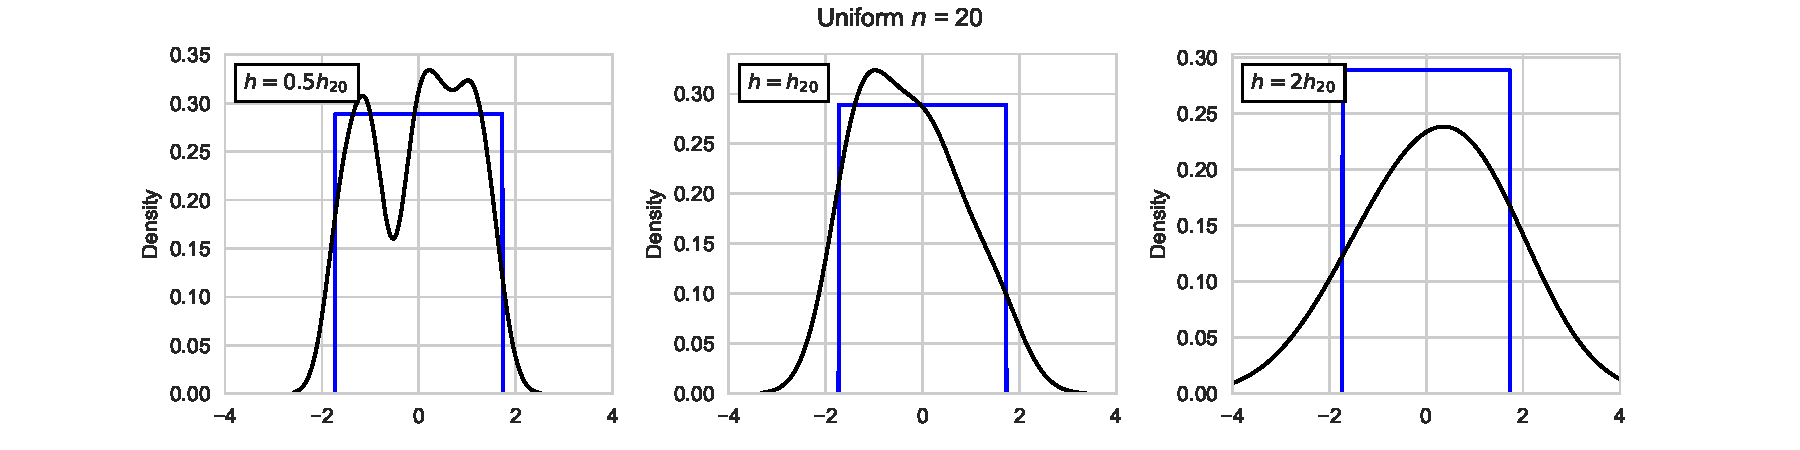
\includegraphics[width = 16 cm]{sources/unifKde20.pdf}
    \caption{Равномерное распределение \eqref{uniform}, $n = 20$}
    \label{fig:uniformKDE20}
\end{figure}
\begin{figure}[H]
    \centering
    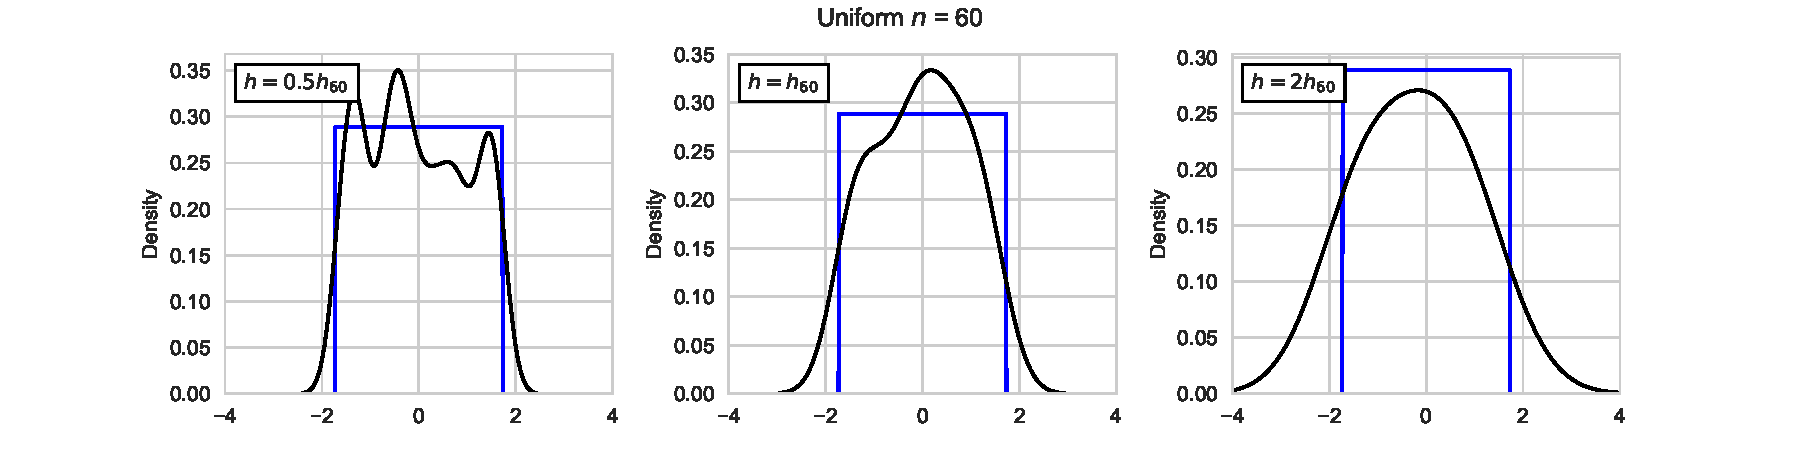
\includegraphics[width = 16 cm]{sources/unifKde60.pdf}
    \caption{Равномерное распределение \eqref{uniform}, $n = 60$}
    \label{fig:uniformKDE60}
\end{figure}
\begin{figure}[H]
    \centering
    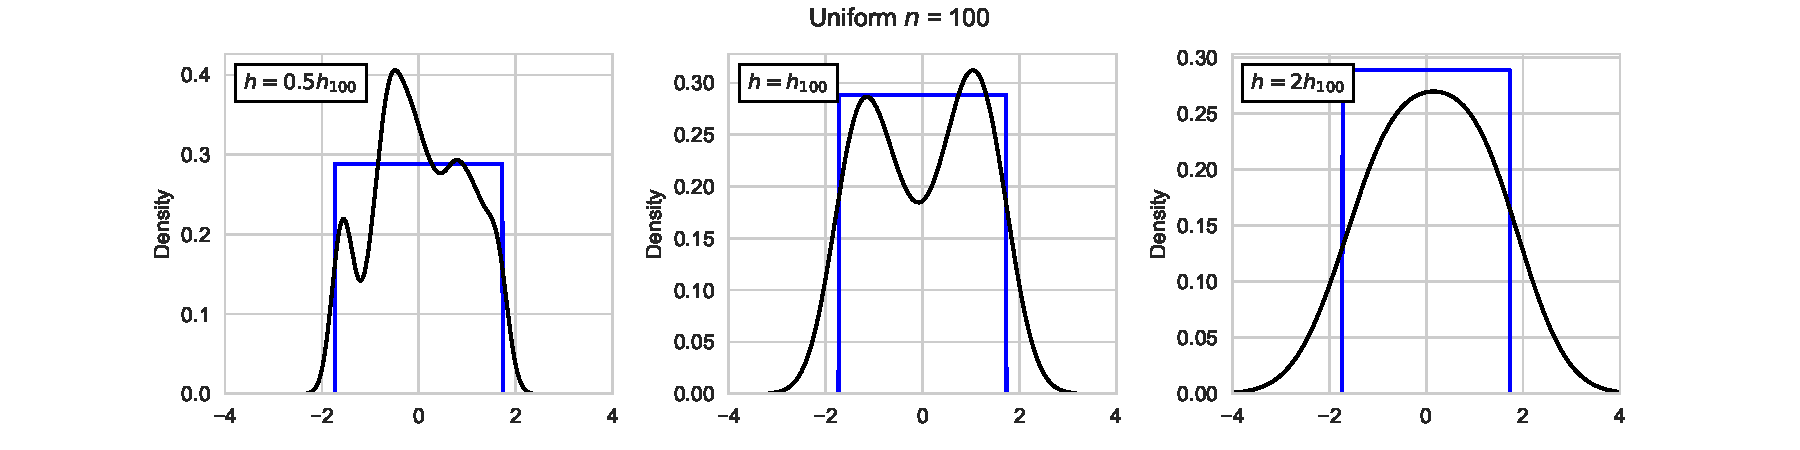
\includegraphics[width = 16 cm]{sources/unifKde100.pdf}
    \caption{Равномерное распределение \eqref{uniform}, $n = 100$}
    \label{fig:uniformKDE100}
\end{figure}
\section{Обсуждение}
\subsection{Гистограмма и график плотности распределения}
Результаты проделанной работы указывают на то, что для каждого из распределений справедливо следующее замечание: при увеличении количества элементов выборки ее гистограмма становится ближе к графику плотности вероятности того закона, по которому распределены эти элементы. Чем меньше выборка, тем менее она репрезентативна и тем хуже по ней определяется характер распределения исследуемой величины.\\
\\
В большинстве случаев максимумы гистограмм и плотностей распределения не совпали. В некоторых местах прослеживаются всплески гистограмм, наиболее отчетливо - на распределении Коши.
\subsection{Характеристики положения и рассеяния}
В полученных данных, приведенных в таблице, особый интерес представляет дисперсия характеристик рассеяния для распределения Коши, чьи значения можно назвать аномально большими. Ясно, что это результат выбросов, которые можно было наблюдать в результатах предыдущего задания.
\subsection{Доля и теоретическая вероятность выбросов}
Исходя из данных в таблице, можно сделать вывод о том, что при увеличении размеров выборки доля выбросов в ней стремится к теоретической оценке. Самая высокая доля выбросов среди всех распределений наблюдается для распределения Коши. При увеличении выборки равномерное распределение показывает стремительный рост к теоретической оценке - выбросы практически не наблюдаются.\\\\
Ящики с <<усами>> в удобной форме показывает многие важные характеристики выборки (медиана, первый и третий квартили, т.д.), из которых можно делать выводы касательно природы входных данных.
\subsection{Эмпирическая функция и ядерные оценки плотности распределения}
Из графиков видно, что при увеличении размеров выборки э. ф. р. этой выборки приближается к функции распределения того закона, по которому распределены её элементы. Наибольшее отклонение э. ф. р. от реальной функции распределения наблюдается при рассмотрении распределения Пуассона.\\\\
В случае же с ядерными оценками можно сделать вывод о постепенном сближении ядерной оценки и функции плотности вероятности при увеличении размеров выборки при любом выборе $h$.\\\\
В зависимости от особенностей распределений для их описания лучше подходят разные параметры $h$ в ядерной оценке. Правильный выбор такого значения дает вид ядерной оценки, наиболее близкий к плотности данного распределения.\\\\
С ростом числового коэффициента при $h_n$ уменьшается число чередований знака производной аппроксимирующей функции на рассматриваемом промежутке, её характер становится все более унимодальным.
\section*{Примечание}
С кодом работы и отчета можно ознакомиться по ссылкам:\\\url{https://github.com/Kozlov992/MS2021/tree/master/Labs1-2}
\end{document}
